\chapter{Experimental Results}

\section{ICP registration}

\subsection{Resolutions and \gls{icp} result, Bunny model} \label{sec:ex_bunny_hilo}
\begin{tabularx}{\textwidth}{|r|X|} \hline
Method & ICP. Select all points, closest point criterion, equal weights, no rejection, point-to-point error metric. \\ \hline
Model & Stanford Bunny model. \\ \hline
Fixed & 50\% of model points, randomly chosen. \\ \hline
Loose & Starting from the other 50\%, randomly downsampled by given amount. $60$ steps. \\ \hline
Displacement & See captions on the figures. \\ \hline
Y Axis & True error, after $40$ iterations. \\\hline
X Axis & Number of points in Loose divided by number of points in Fixed. Lower value means Loose has lover resolution. \\ \hline
\end{tabularx}

\subsubsection{No displacement}
The two point clouds are perfectly aligned to start with.

\begin{figure}[H]
\centering
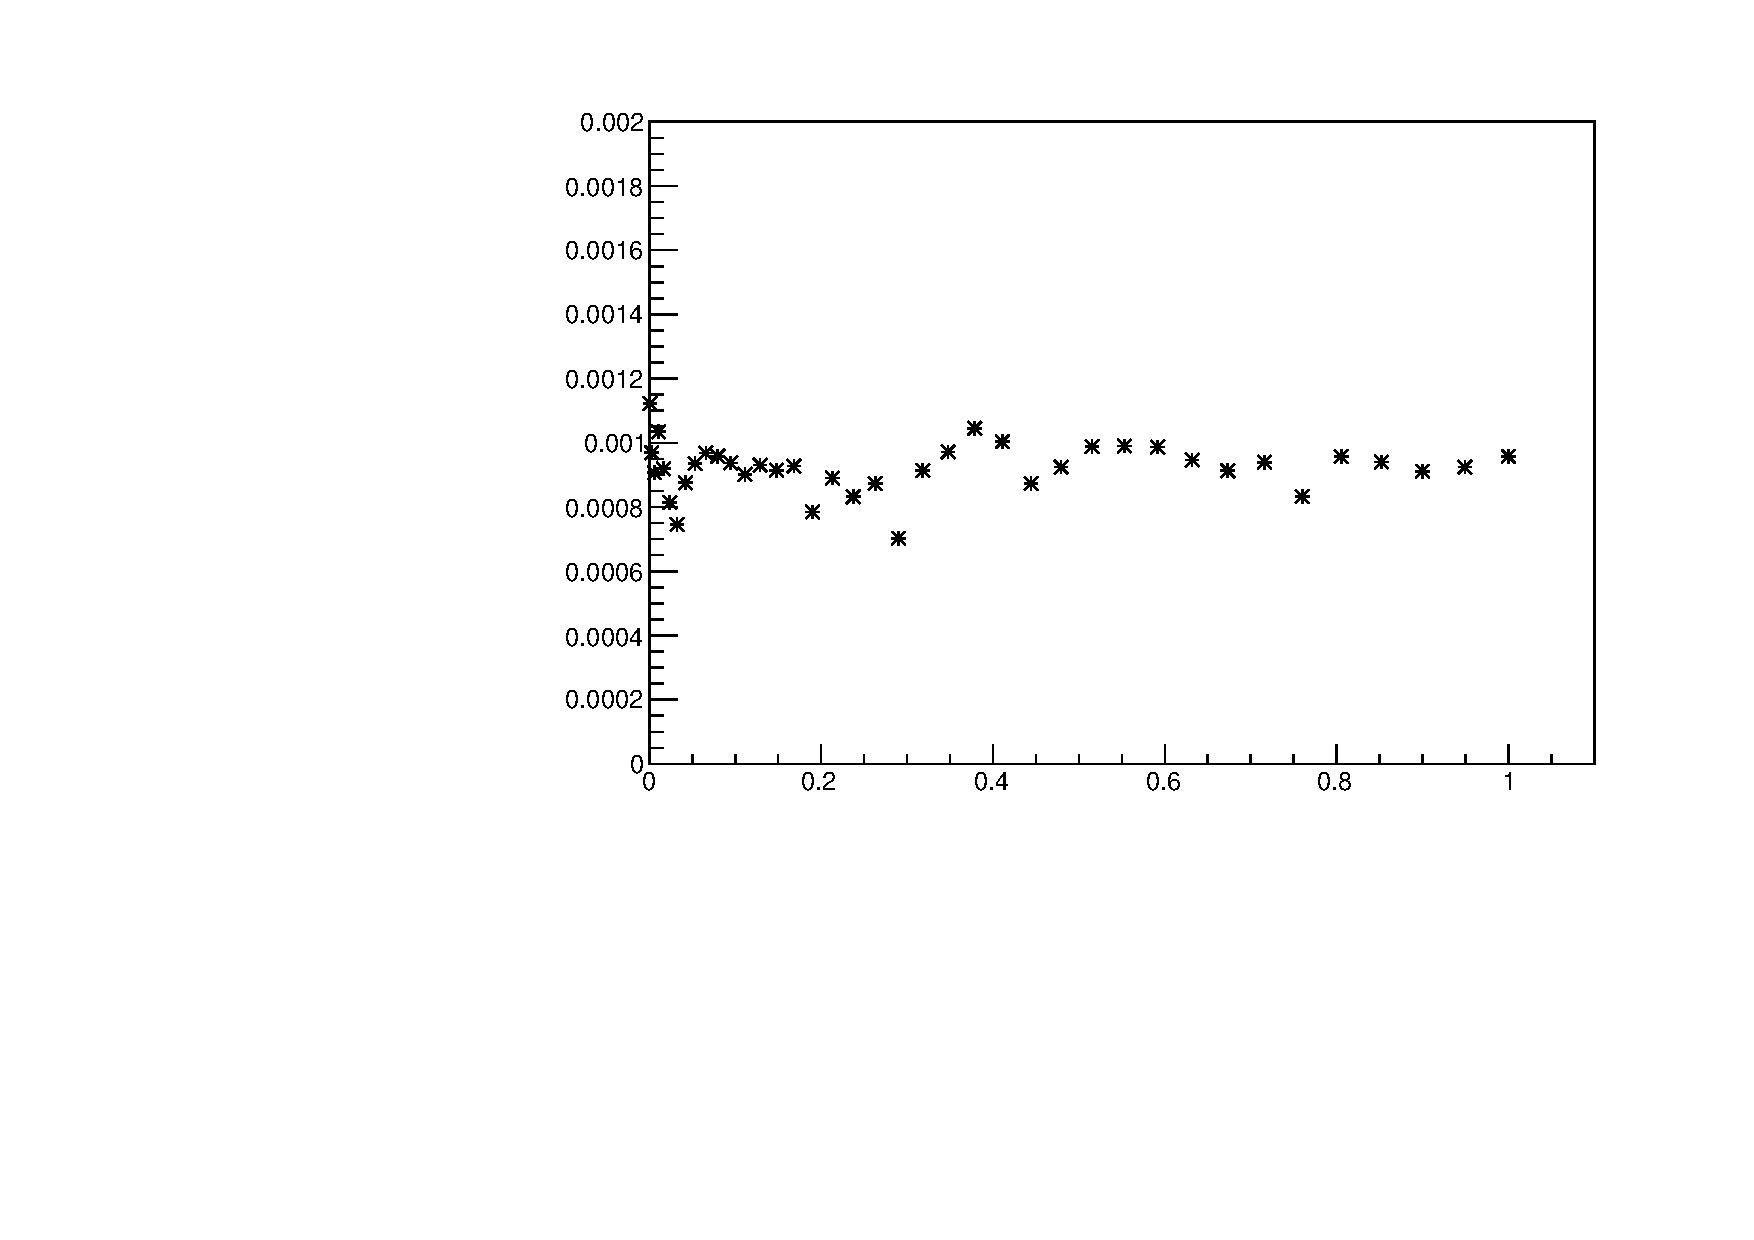
\includegraphics[width=.7\textwidth]{fig/bunny_globmin.pdf}
\caption{no displacement}
\label{fig:bunny_globmin}
\end{figure}

\subsubsection{Small displacement}
Small displacement. Translation by magnitude of $0.01$ in random direction, rotation by $3 \si{\degree}$ or $15 \si{\degree}$ on random axis direction. The Bunny modes has a width, height and depth of about $0.15$.

\begin{figure}[H]
\centering
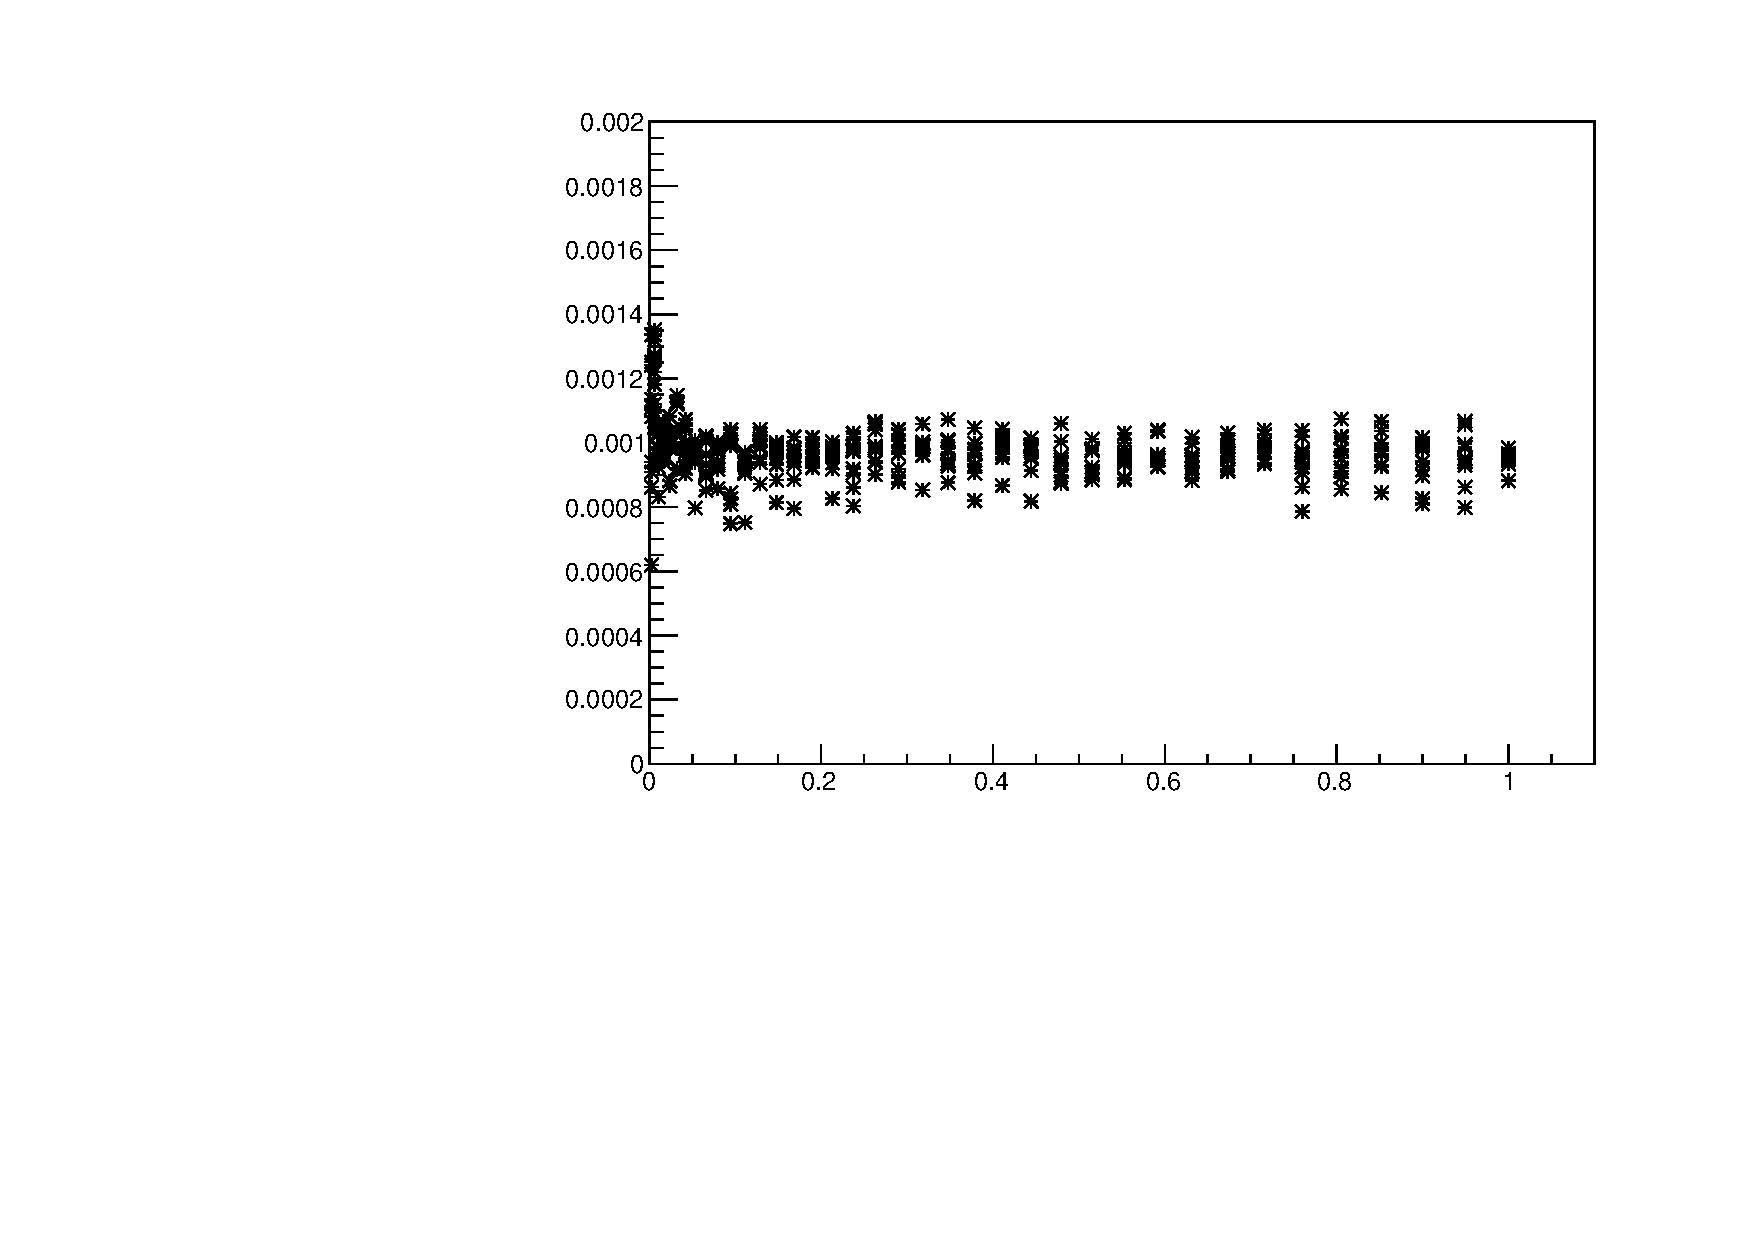
\includegraphics[width=.7\textwidth]{fig/bunny_globsmall.pdf}
\caption{random translation of $0.01$ and rotation of $3 \si{\degree}$, chosen $10$ times}
\label{fig:bunny_globsmall}
\end{figure}

\begin{figure}[H]
\centering
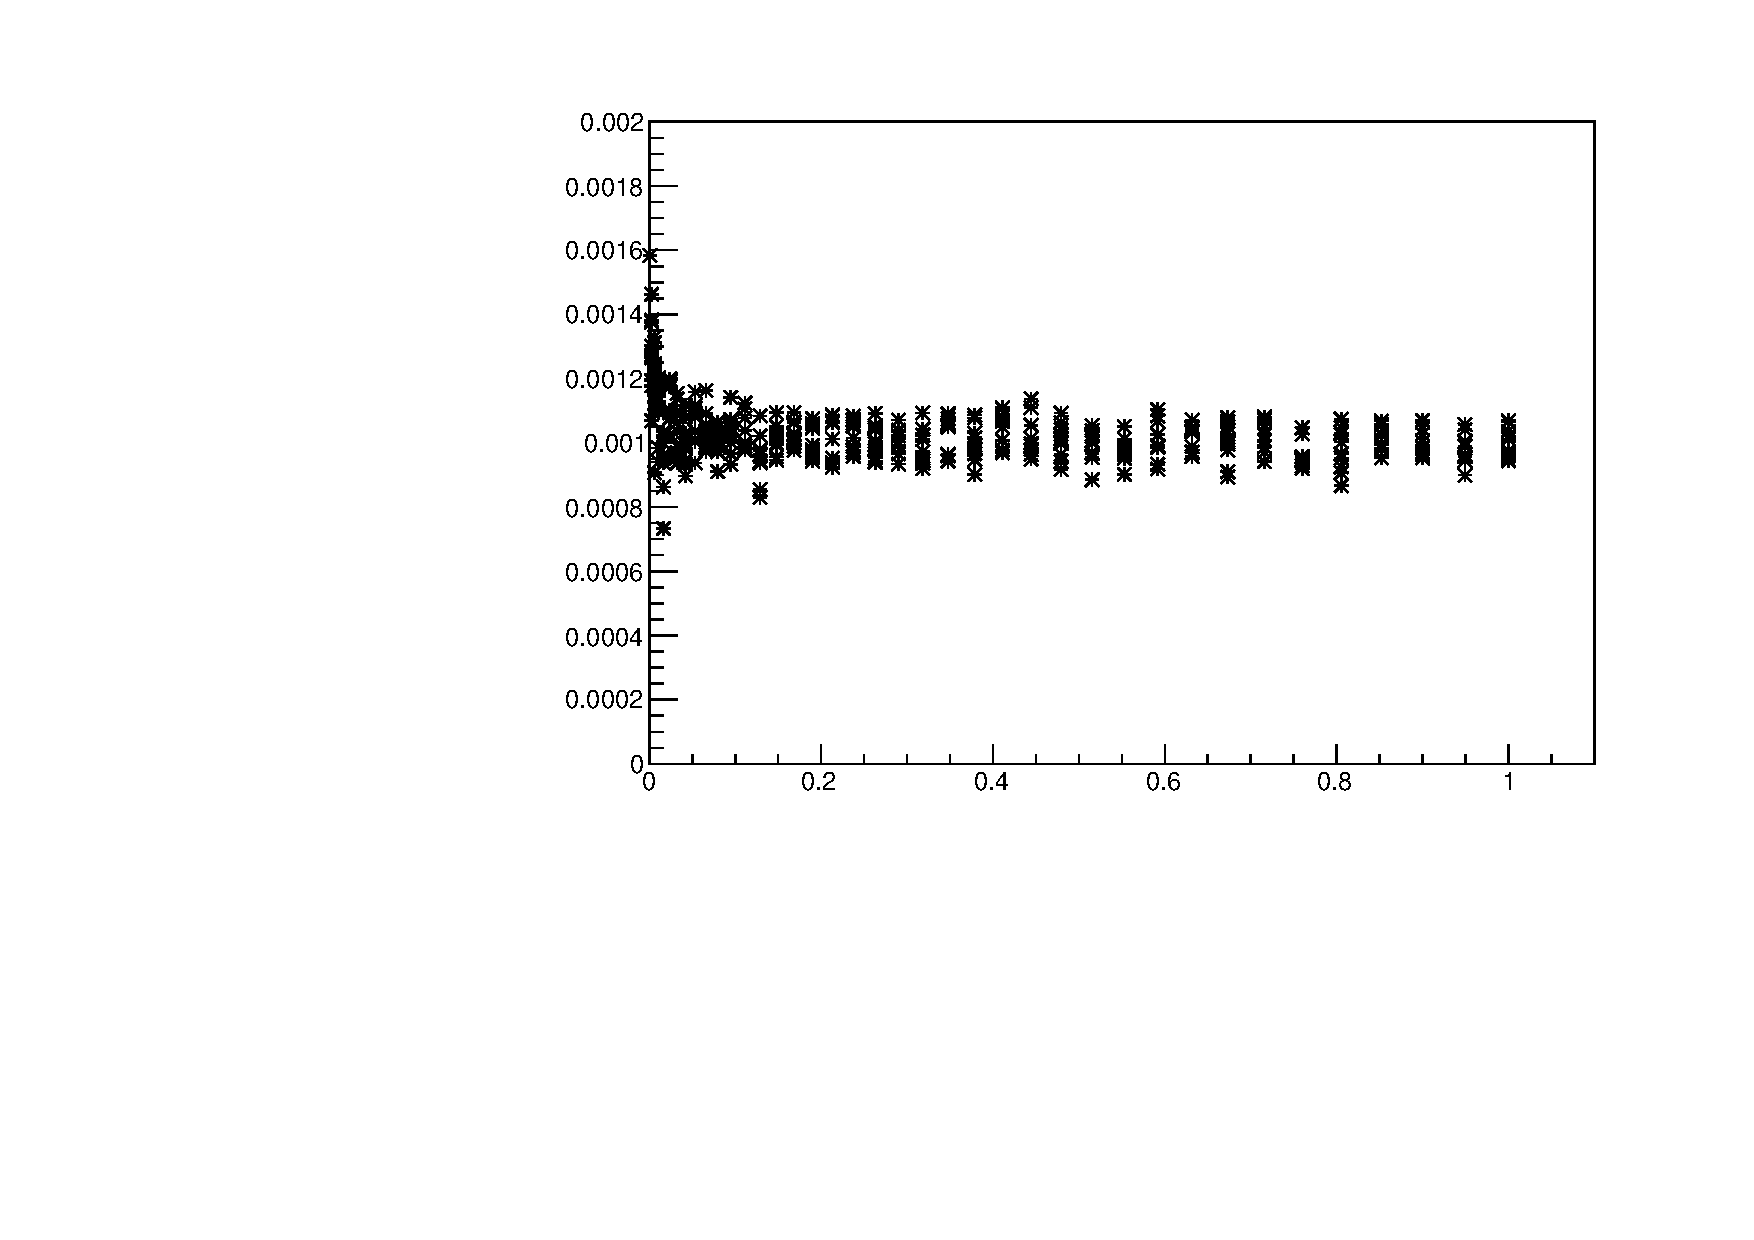
\includegraphics[width=.7\textwidth]{fig/bunny_globmed.pdf}
\caption{random translation of $0.01$ and rotation of $15 \si{\degree}$, chosen $10$ times}
\label{fig:bunny_globmed}
\end{figure}

\subsection{Evolution of \gls{icp} registration, Bunny model}
This plot shows the evolution of the true error \gls{icp} registration, for the same input point clouds. Initially the point clouds are perfectly aligned. The Loose point clouds is randomly generated as before, results from all $60$ registration runs are superimposed.

\begin{tabularx}{\textwidth}{|r|X|} \hline
Method & ICP. Select all points, closest point criterion, equal weights, no rejection, point-to-point error metric. \\ \hline
Model & Stanford Bunny model. \\ \hline
Fixed & 50\% of model points, randomly chosen. \\ \hline
Loose & Starting from the other 50\%, randomly downsampled by given amount. $60$ steps. \\ \hline
Displacement & No displacement. \\ \hline
Y Axis & True error at iteration $i$. \\\hline
X Axis & Iteration step $i$. \\ \hline
\end{tabularx}

\begin{figure}[H]
\centering
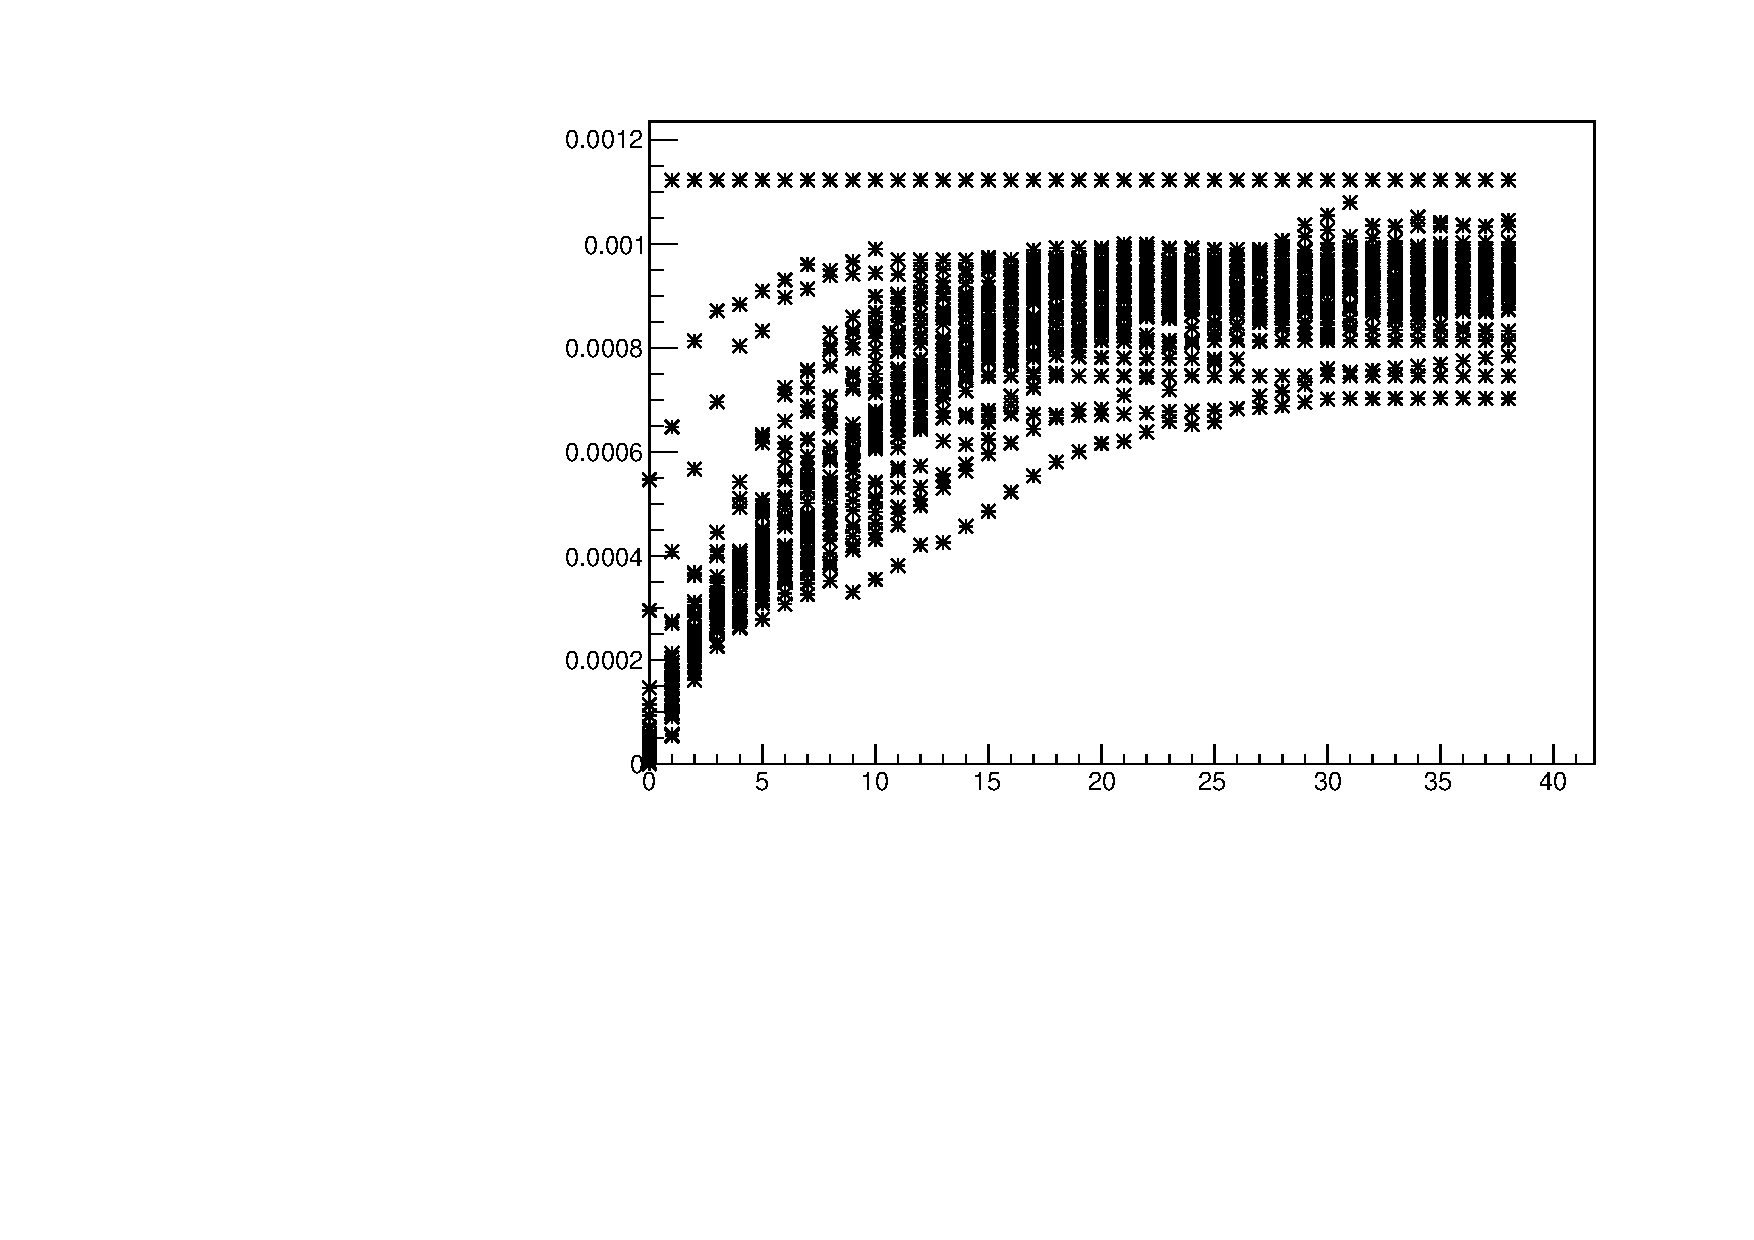
\includegraphics[width=.7\textwidth]{fig/bunny_globmin_ev.pdf}
\caption{Evolutions of true error for experiment \ref{ref:bunny_hilo_a}}
\label{fig:bunny_hilo_ev}
\end{figure}


\subsection{Resolutions and \gls{icp} result, sphere model} \label{sec:ex_sphere_hilo}
\begin{tabularx}{\textwidth}{|r|X|} \hline
Method & ICP. Select all points, closest point criterion, equal weights, no rejection, point-to-point error metric. \\ \hline
Model & Artificially generated sphere point cloud with random point dispersion. \\ \hline
Fixed & Randomly chosen number of points from $0$ to $50000$. $30$ steps. \\ \hline
Loose & Randomly chosen number of points from $0$ to $50000$. $30$ steps. \\ \hline
Displacement & No displacement. \\ \hline
Y Axis & True error, after $40$ iterations. \\\hline
X Axis & Maximum of number of points in Loose and number of points in Fixed. \\ \hline
\end{tabularx}

\begin{figure}[H]
\centering
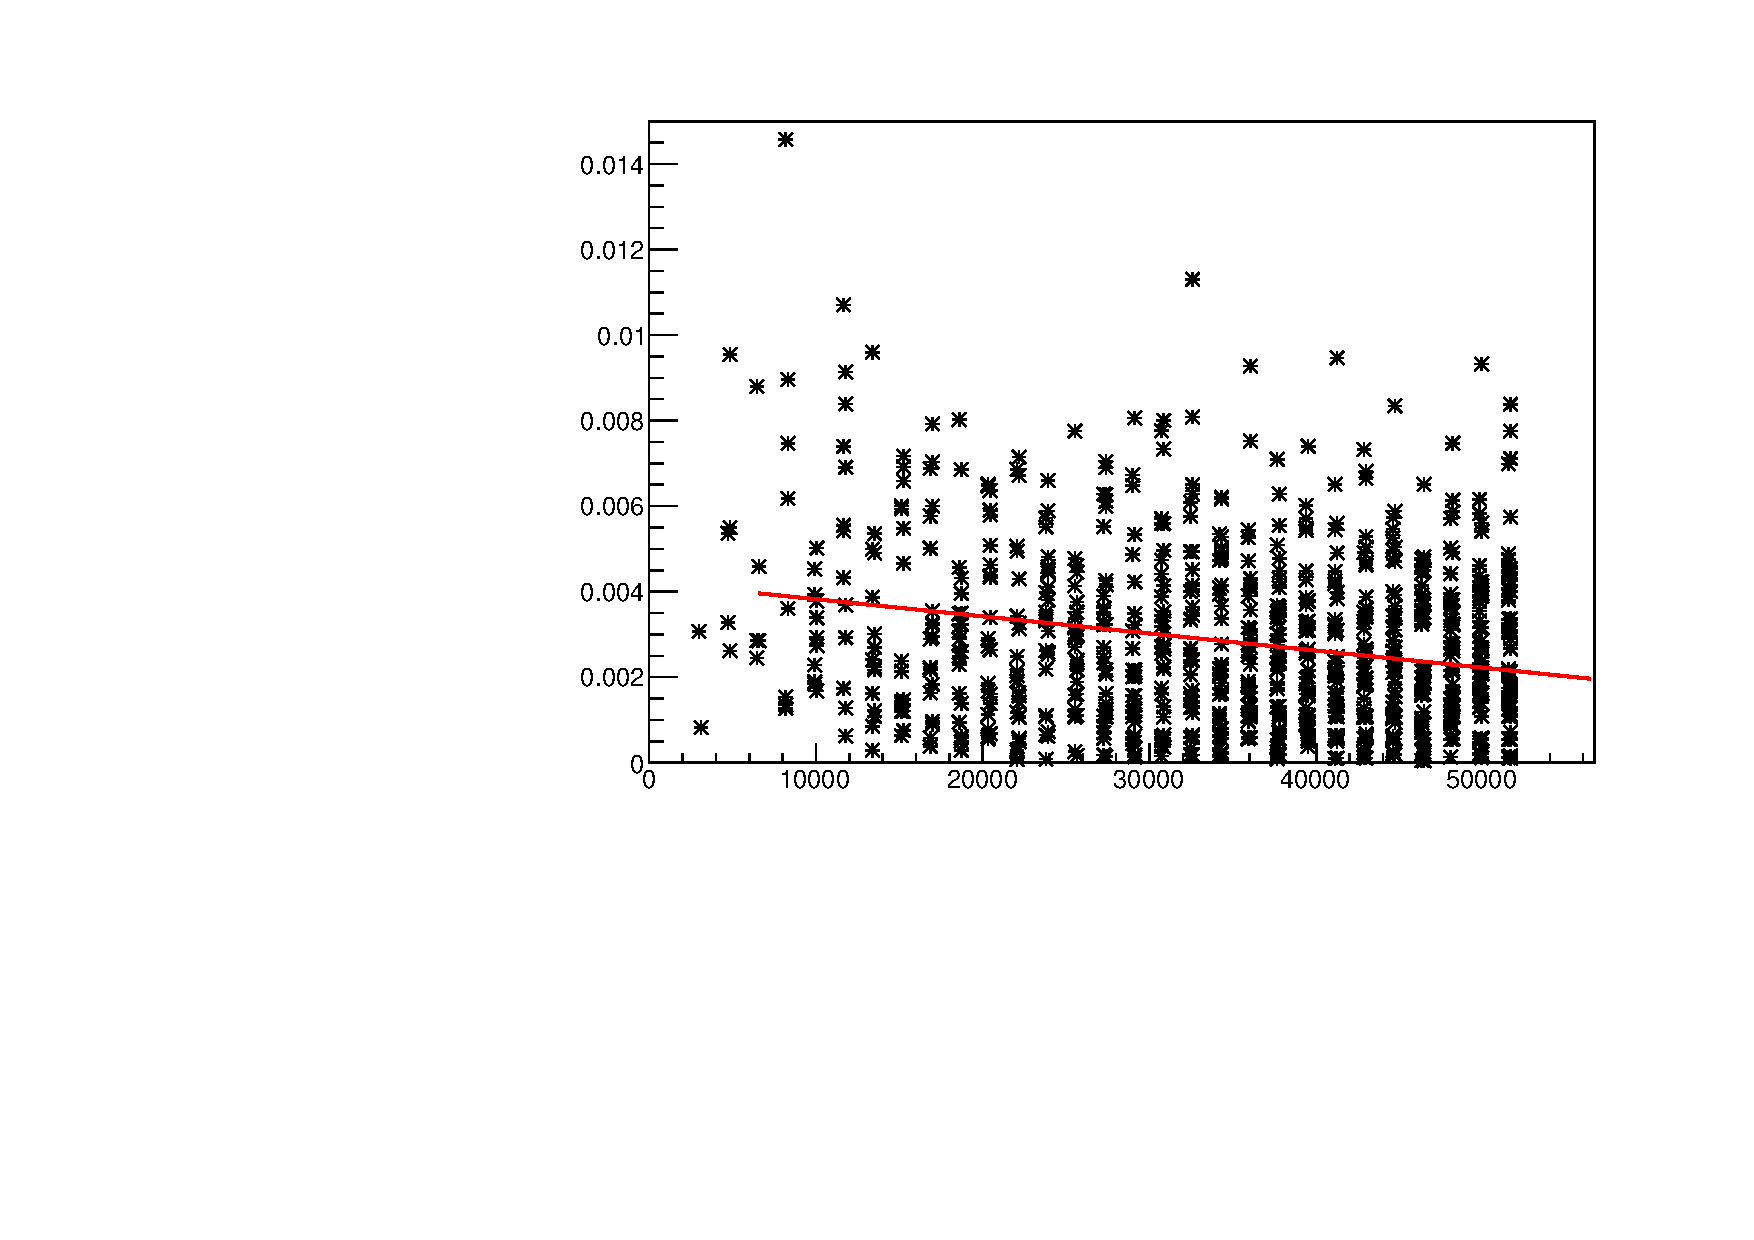
\includegraphics[width=.7\textwidth]{fig/sphere_icp.pdf}
\end{figure}


\subsection{View-point and \gls{icp} result, relief model} \label{sec:ex_relief_dproj}

\begin{tabularx}{\textwidth}{|r|X|} \hline
Method & ICP. Select all points, closest point criterion, equal weights, no rejection, point-to-point error metric. \\ \hline
Model & Relief point cloud, projected with occlusion from camera placed at angle looking down on relief. \\ \hline
Fixed & Point cloud of relief with camera angle varying in $[0, 2 \pi]$ around relief. $20$ steps. \\ \hline
Loose & Point cloud of relief with camera angle varying in $[0, 2 \pi]$ around relief. $20$ steps. \\ \hline
Displacement & No displacement. \\ \hline
Y Axis & True error, after $40$ iterations. \\\hline
X Axis & Angle between Fixed and Loose camera positions. \\ \hline
\end{tabularx}

\begin{figure}[H]
\centering
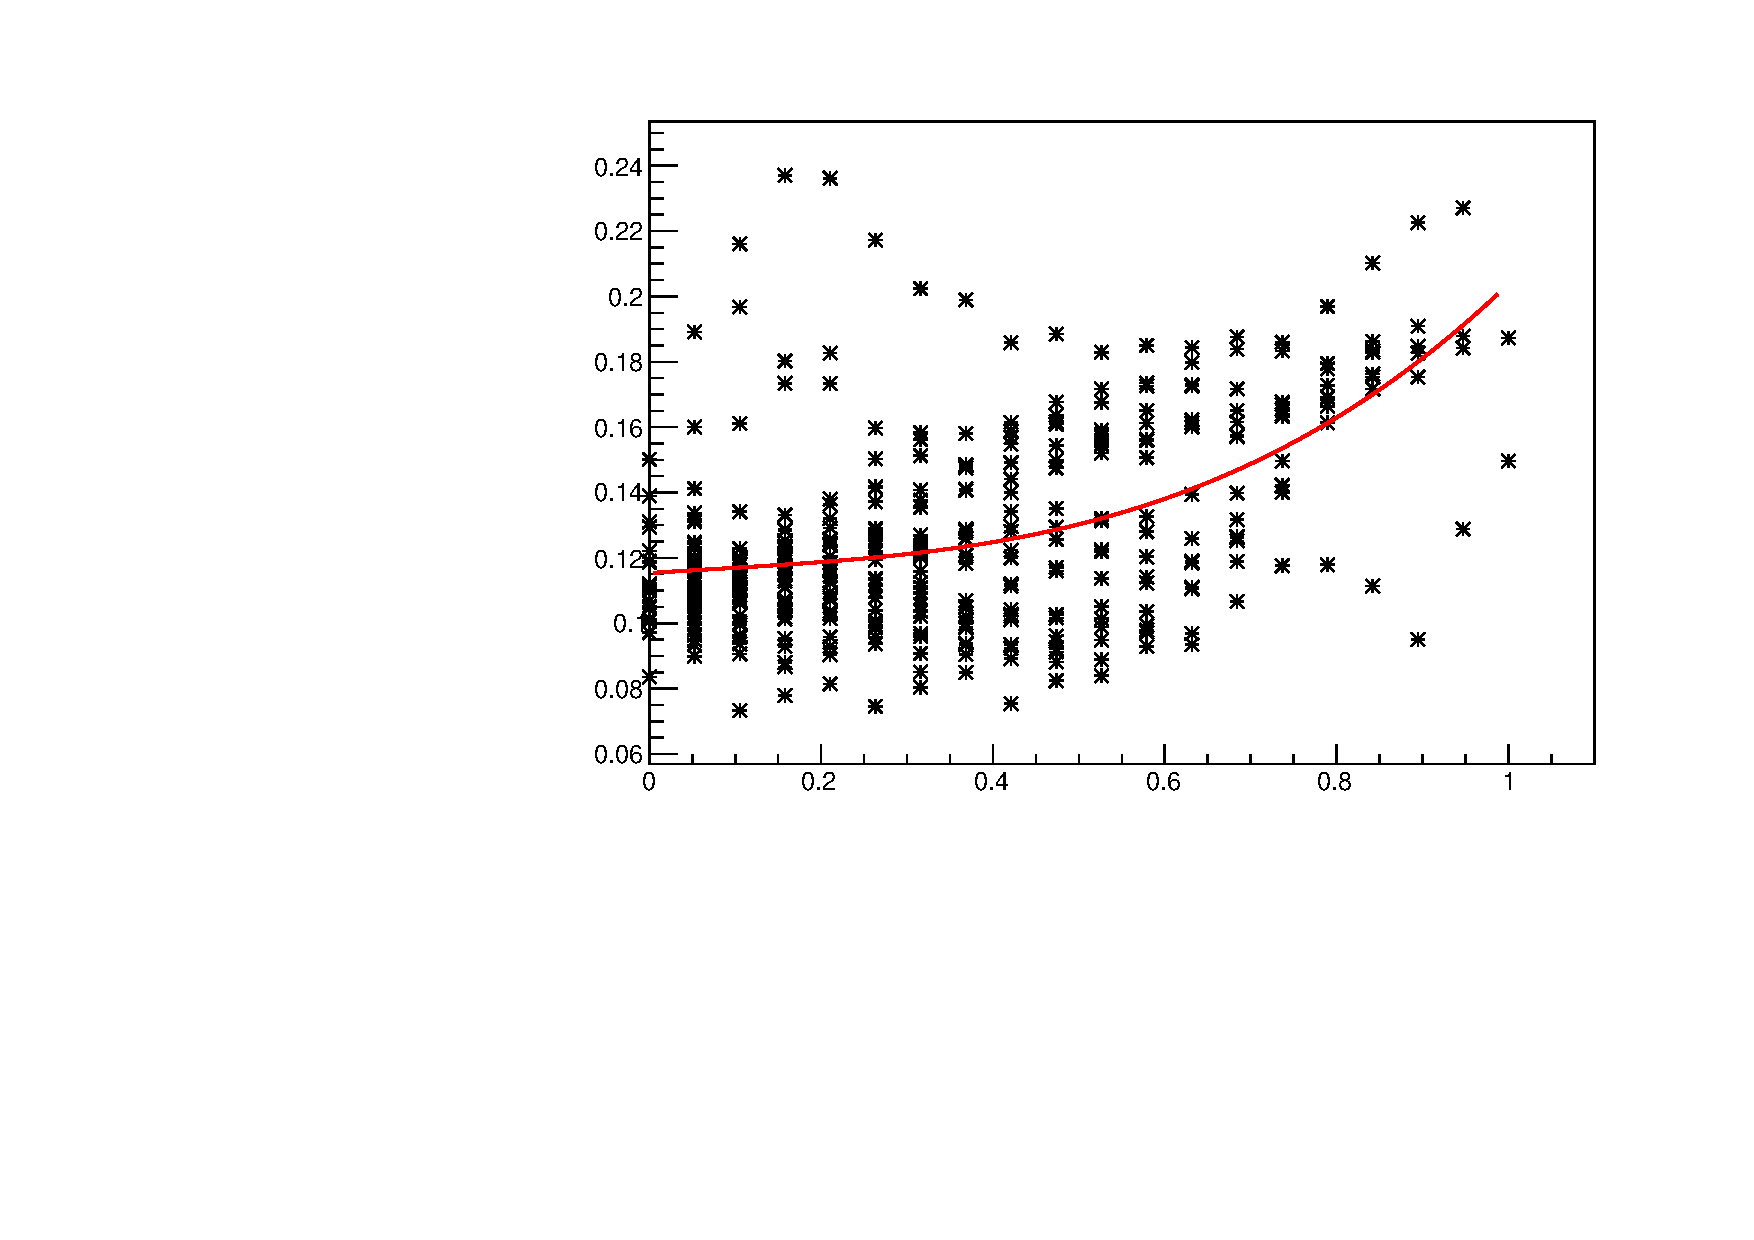
\includegraphics[width=.7\textwidth]{fig/relief_dproj.pdf}
\end{figure}


\newpage


\section{Relief small transformation \gls{acdh}} \label{sec:relief_small_trans_exp}
The following figures depict \gls{acdh} of a relief point cloud $P$ like the one on figure \ref {fig:relief_plain}, on which a small transformation $\matr{M}$ was applied. For the point cloud $P$, the average nearest neighbor distance on surfaces perpendicular to the camera ray is $p_l = 0.01$. The plane of the relief is along the X and Y axis.

\subsection{Translations}
Translations are applied on two axis, by the amounts \{ 0, 0.002, 0.004, 0.006, 0.008, 0.010 \}.

\subsubsection{X and Y axis} \label{sec:res_acdh_txy}
Here $\matr{M}$ is a translation in X and Y axis, by these amounts. No translation in Z axis and no rotation is applied.

The top-left cell shows the own distance histogram, where $\matr{M} = \matr{I}$. Only translations in the positive directions are made, translations in the negative directions would yield similar results.

\begin{figure}[H]
\foreach \y in {0,1,2,3,4} {
	\foreach \x in {0,1,2,3,4} {
		\includegraphics[width=0.19\linewidth]{fig/cross_relief_trans/(\x-\y-0).pdf}
	}
	\\
}
\caption{Horizontal: X translation, vertical: Y translation}
\end{figure}

\paragraph{Observations}
Translation on the X and on the Y axis have similar results, which is to be expected since the plane of the relief spans in those directions. If $P$ was a perfect plane, the histograms would retain exactly the same shape. Because this is not the case, distances between points on more oblique parts of the surface are increased, resulting in a slightly more convex curvature.

\subsubsection{X and Z axis} \label{sec:res_acdh_txz}
Y axis translation fixed to $0$. Translations by same amounts.

\begin{figure}[H]
\foreach \z in {0,1,2,3,4} {
	\foreach \x in {0,1,2,3,4} {
		\includegraphics[width=0.19\linewidth]{fig/cross_relief_trans/(\x-0-\z).pdf}
	}
	\\
}
\caption{Horizontal: X translation, vertical: Z translation}
\label{fig:ex_trans_xz}
\end{figure}

\paragraph{Observations}
Translation on the X axis is the same as before. But the translation on the Z axis pulls the surfaces, and the histogram gets an offset to the right side. Some oblique surfaces of the model remain close, explaining that parts of the linear increase can remain unchanged.

\newpage


\subsection{Rotations}
Here instead of a translation, a rotation gets applied on the same point cloud. The point of rotation is the center point of the relief plane. The amounts of rotation are \{ 0, 1\si{\degree}, 2\si{\degree}, 3\si{\degree}, 4\si{\degree}, 5\si{\degree} \}.

\subsubsection{Rotation around X and Y axis} \label{sec:res_acdh_rxy}
\begin{figure}[H]
\foreach \y in {0,1,2,3,4} {
	\foreach \x in {0,1,2,3,4} {
		\includegraphics[width=0.19\linewidth]{fig/cross_relief_rot/(\x-\y-0).pdf}
	}
	\\
}
\caption{Horizontal: X axis rotation, vertical: Y axis rotation}
\end{figure}

\paragraph{Observations}
When the point cloud is rotated along the center point, distances of points change more, the further the points are from the center. Because less distances are recorded within the range $[0, \frac{1}{2} l_{\text{min}}]$, the adjusted histogram becomes more jagged.


\subsubsection{Rotation around X and Z axis} \label{sec:res_acdh_rxz}
\begin{figure}[H]
\foreach \z in {0,1,2,3,4} {
	\foreach \x in {0,1,2,3,4} {
		\includegraphics[width=0.19\linewidth]{fig/cross_relief_rot/(\x-0-\z).pdf}
	}
	\\
}
\caption{Horizontal: X axis rotation, vertical: Z axis rotation}
\end{figure}

\paragraph{Observations}
The results are similar as before. The increase in jaggedness is weaker for rotations on the Z axis, because a larger part of the surfaces do not get pulled off each other but slide on each other.



\newpage


\section{Relief small transformation \gls{arcdh}}
Here the same translations are rotations are applied, and the \gls{arcdh} instead of the \gls{acdh} is shown.

\subsection{Translations}

\subsubsection{Translation in X and Y axis} \label{sec:res_arcdh_txy}

\begin{figure}[H]
\foreach \y in {0,1,2,3,4} {
	\foreach \x in {0,1,2,3,4} {
		\includegraphics[width=0.19\linewidth]{fig/cross_relief_trans_rej/(\x-\y-0).pdf}
	}
	\\
}
\caption{Horizontal: X translation, vertical: Y translation}
\end{figure}

\paragraph{Observations}
The histograms remain unchanged. In comparison to \ref{sec:res_acdh_txy}, the effect of the oblique surfaces get cancelled out because points are projected back onto the surface after the translation.

\subsubsection{Translation in X and Z axis} \label{sec:res_arcdh_txz}

\begin{figure}[H]
\foreach \z in {0,1,2,3,4} {
	\foreach \x in {0,1,2,3,4} {
		\includegraphics[width=0.19\linewidth]{fig/cross_relief_trans_rej/(\x-0-\z).pdf}
	}
	\\
}
\caption{Horizontal: X translation, vertical: Z translation}
\label{fig:ex_trans_xz_rej}
\end{figure}

\paragraph{Observations}
The histograms also remain unchanged.

\newpage

\subsection{Rotations}

\subsubsection{Rotation around X and Y axis} \label{sec:res_arcdh_rxy}
\begin{figure}[H]
\foreach \y in {0,1,2,3,4} {
	\foreach \x in {0,1,2,3,4} {
		\includegraphics[width=0.19\linewidth]{fig/cross_relief_rot_rej/(\x-\y-0).pdf}
	}
	\\
}
\caption{Horizontal: X axis rotation, vertical: Y axis rotation}
\end{figure}

\paragraph{Observations} It can be observed that the histogram becomes slightly less linear and more jagged with larger rotation angles.


\subsubsection{Rotation around X and Z axis} \label{sec:res_arcdh_rxz}
\begin{figure}[H]
\foreach \z in {0,1,2,3,4} {
	\foreach \x in {0,1,2,3,4} {
		\includegraphics[width=0.19\linewidth]{fig/cross_relief_rot_rej/(\x-0-\z).pdf}
	}
	\\
}
\caption{Horizontal: X axis rotation, vertical: Z axis rotation}
\end{figure}

\paragraph{Observations} Same as for the rotation on X and Y axis.


\newpage

\section{\Gls{acdh} histogram comparison error metric} \label{sec:chi_err}
For all of these tests, a relief point cloud is used. The plots in the first row show the histogram comparison error metric, while second row shows the mean absolute error with the closest point criterion.

The three columns differ by the range of the transformations applied. The maximal rotation and translations are the following:

\begin{figure}[H]
\centering
\begin{tabularx}{.4\textwidth}{|r|X|X|} \hline
scale  & translation & rotation \\ \hline
L      & 0.1         & 2.29\si{\degree} \\
M      & 0.01        & 0.23\si{\degree} \\
S      & 0.001       & 0.023\si{\degree} \\ \hline
\end{tabularx}
\end{figure}

So the plot for M can seen as a zoomed in version of the tenth of the plot for L, around $x = 0$. Same for S and M. However, on each plot, the curves are different random cross sections. The rotation angles are chosen so that a rotation on the X or Y axis results in an average displacement of true corresponding points by about the same about as the listed translation.

In each of the tests, a loose point cloud $Q$ is registered to a fixed point cloud $P$ of the same model, but with different resolution or view-point. $Q$ is the sample point cloud for the histograms and has a higher resolution. A graphic is shown with each test that shows a close-up view of both point dispersions, along with a scale indicating the L, M and S translation lengths.





\subsection{Same}
Here $Q$ only has a slightly higher resolution to $P$. The close-up view \ref{fig:t_scale} shows the density of $P$ (black) and $Q$ (blue), along with the maximal extent of the translations for the three columns. 

\begin{figure}[h]
\center
{
\setlength{\fboxsep}{0pt}%
\setlength{\fboxrule}{0.5pt}%
\fbox{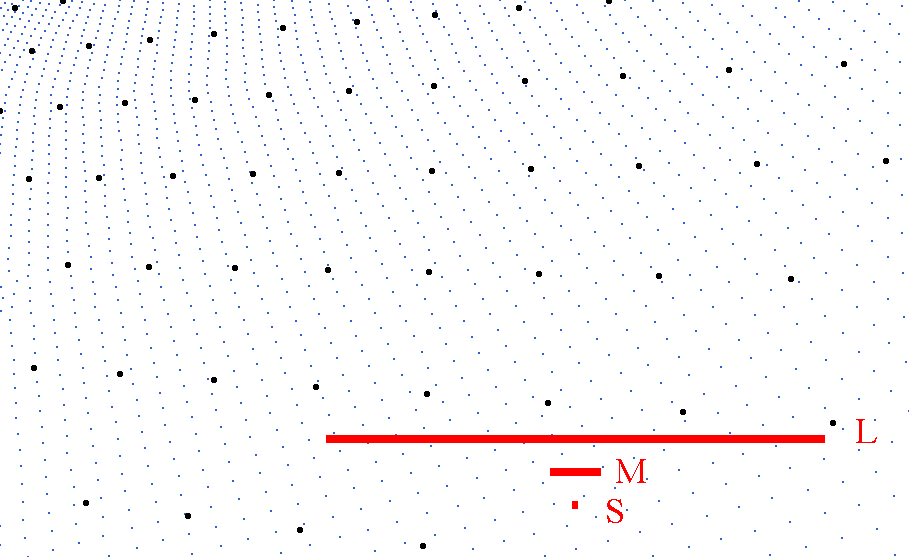
\includegraphics[width=0.4\textwidth]{fig/t_scale.png}}
}
\label{fig:t_scale}
\caption{Close-up view with scale}
\end{figure}

\begin{figure}[H]
\begin{subfigure}{.33\textwidth}
	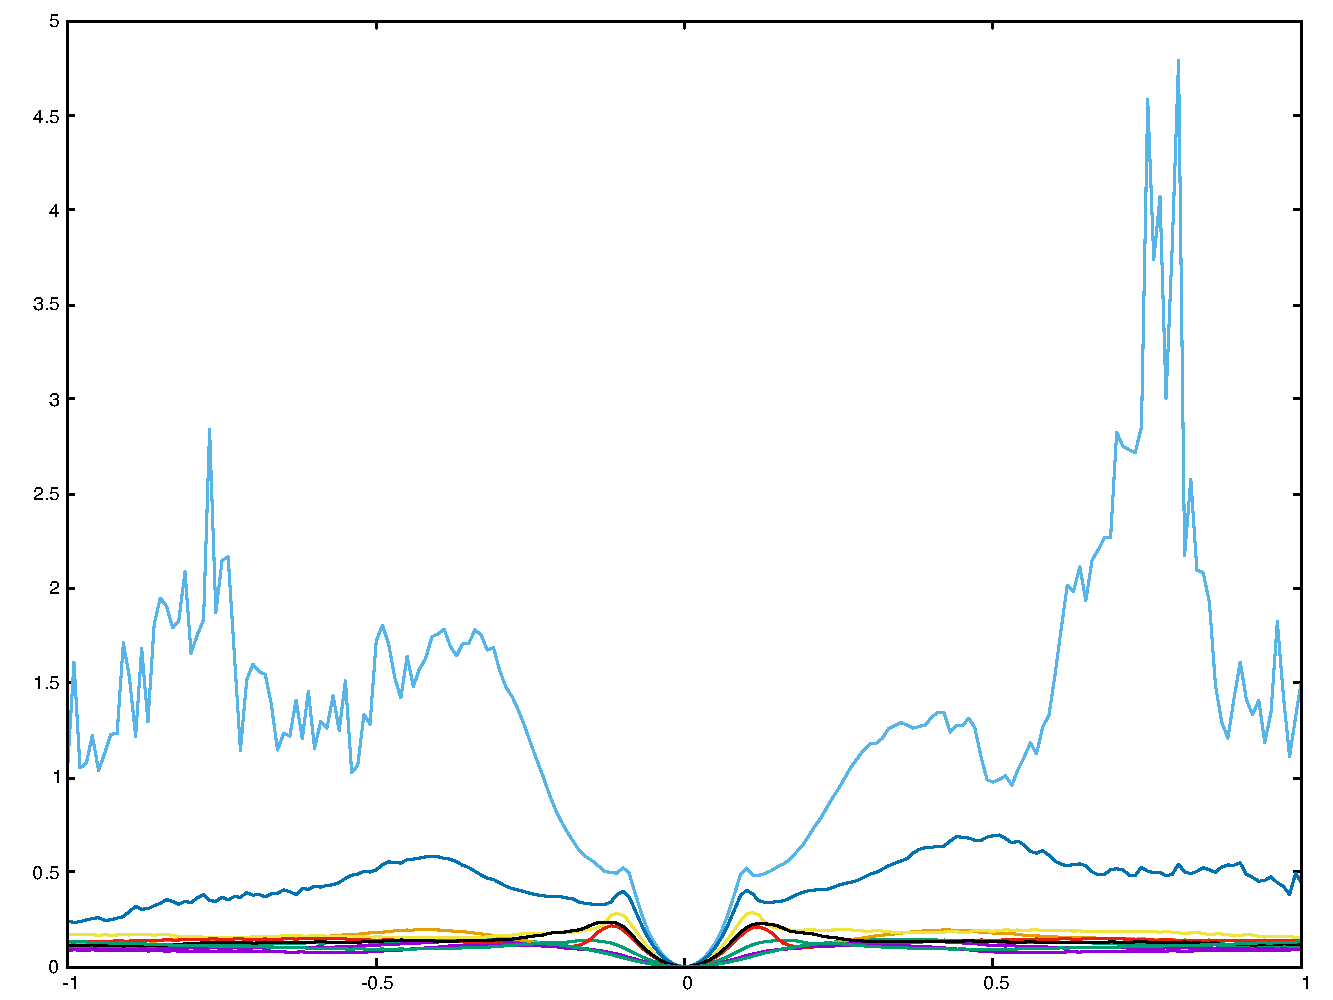
\includegraphics[width=\linewidth]{fig/ajherr/t/L_chi.pdf}
\end{subfigure}%
\begin{subfigure}{.33\textwidth}
	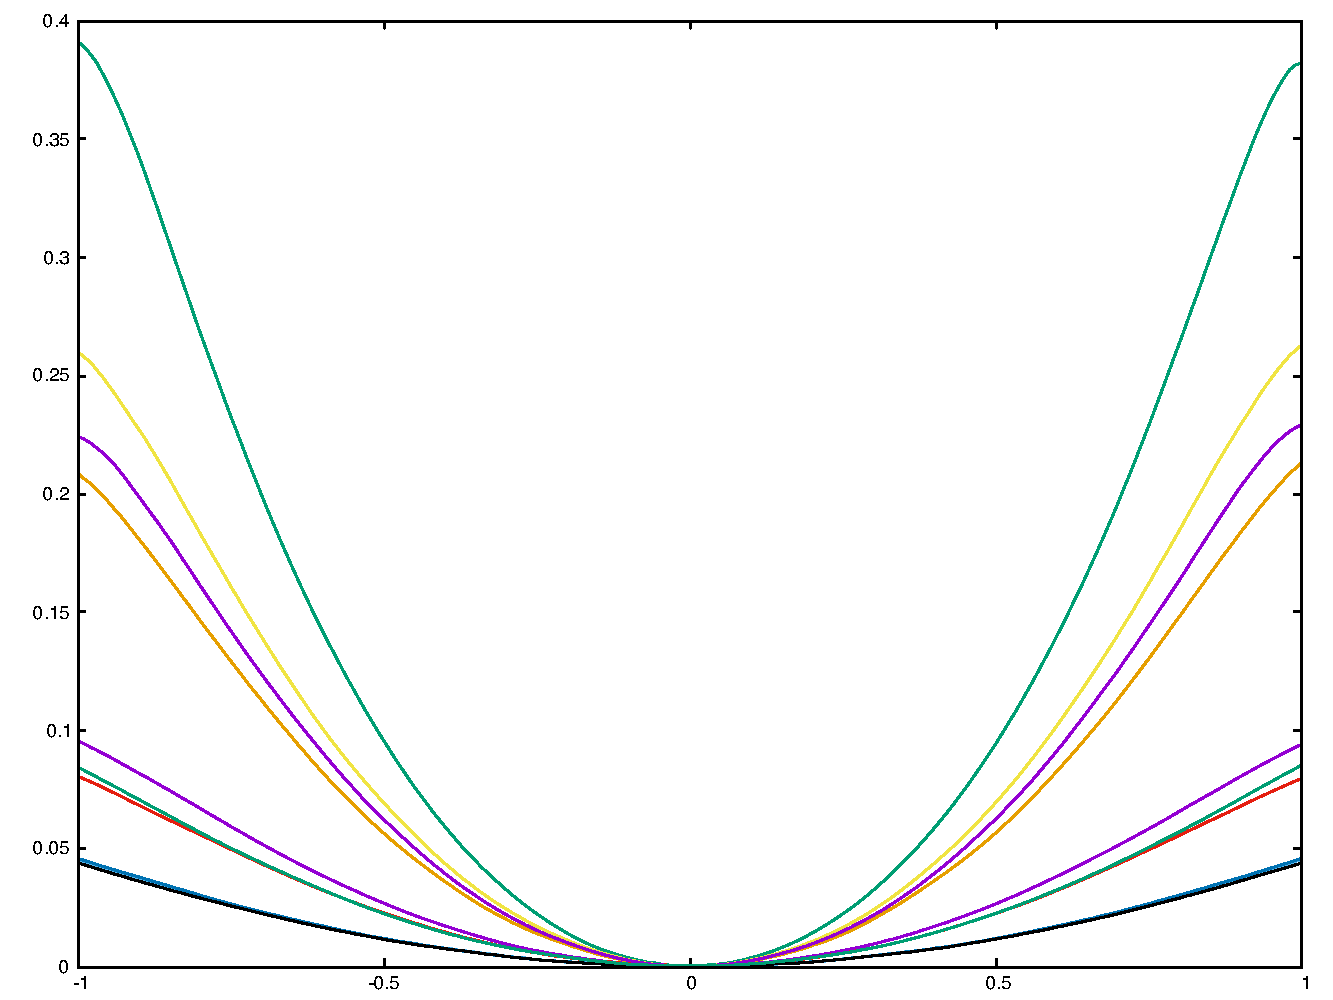
\includegraphics[width=\linewidth]{fig/ajherr/t/M_chi.pdf}
\end{subfigure}&
\begin{subfigure}{.33\textwidth}
	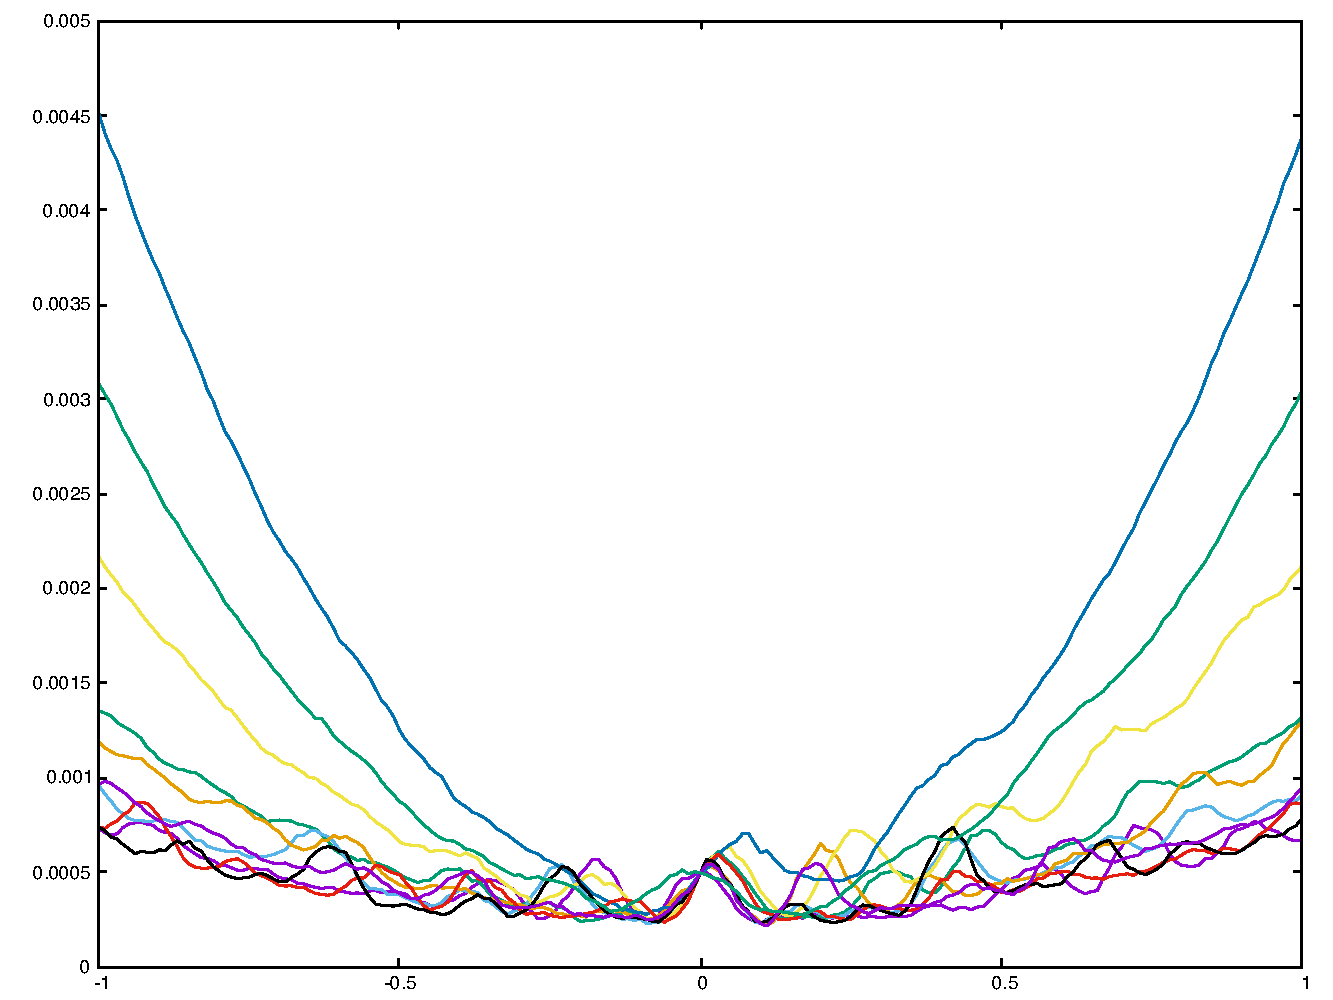
\includegraphics[width=\linewidth]{fig/ajherr/t/S_chi.pdf}
\end{subfigure}\\
\begin{subfigure}{.33\textwidth}
	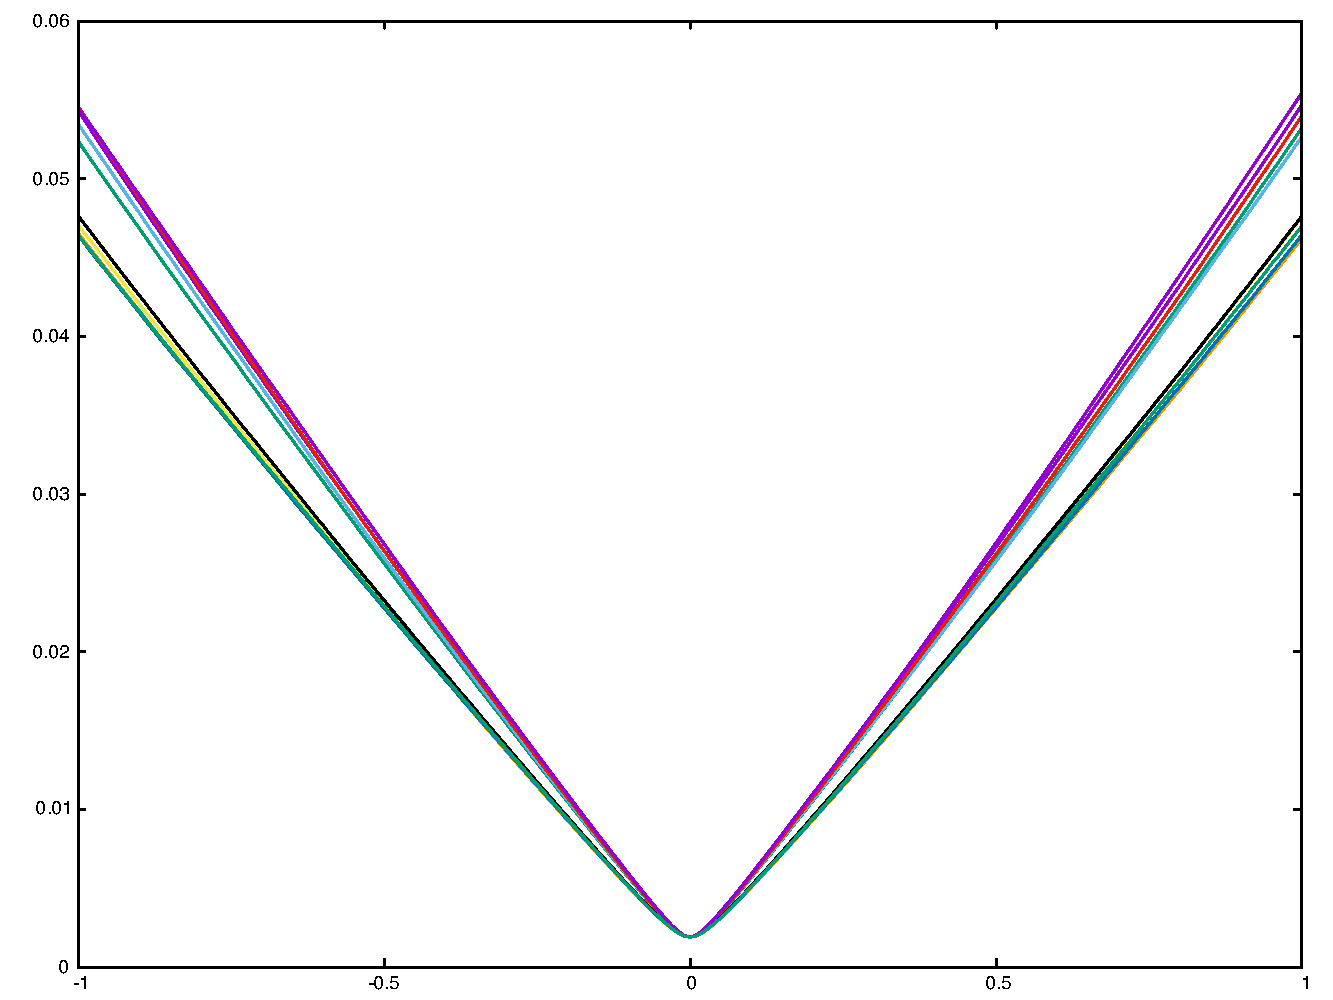
\includegraphics[width=\linewidth]{fig/ajherr/t/L_mae.pdf}
	\caption{L}
\end{subfigure}%
\begin{subfigure}{.33\textwidth}
	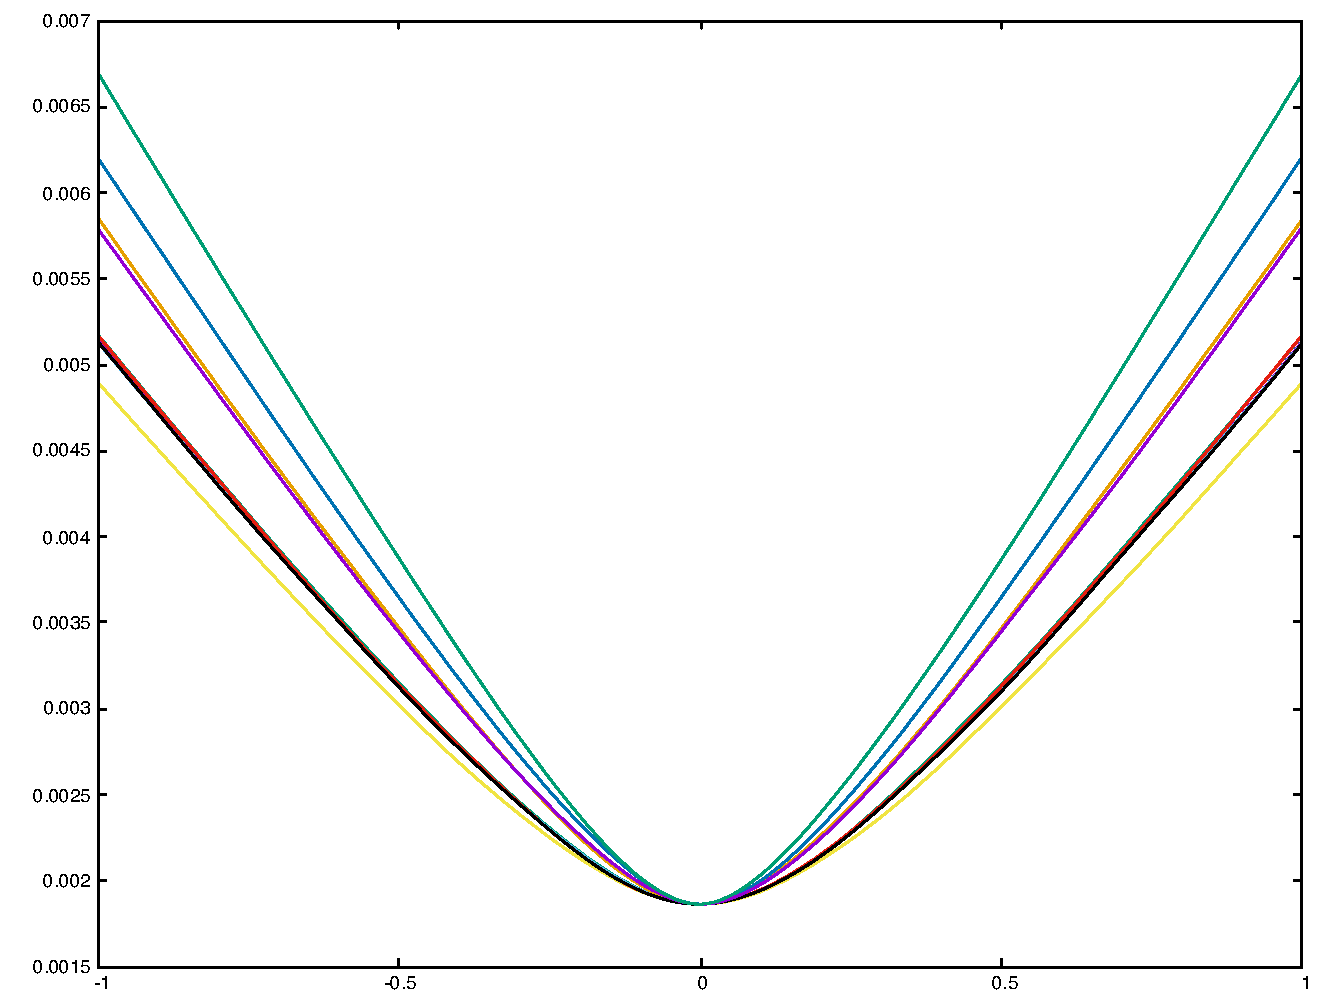
\includegraphics[width=\linewidth]{fig/ajherr/t/M_mae.pdf}
	\caption{M}
\end{subfigure}&
\begin{subfigure}{.33\textwidth}
	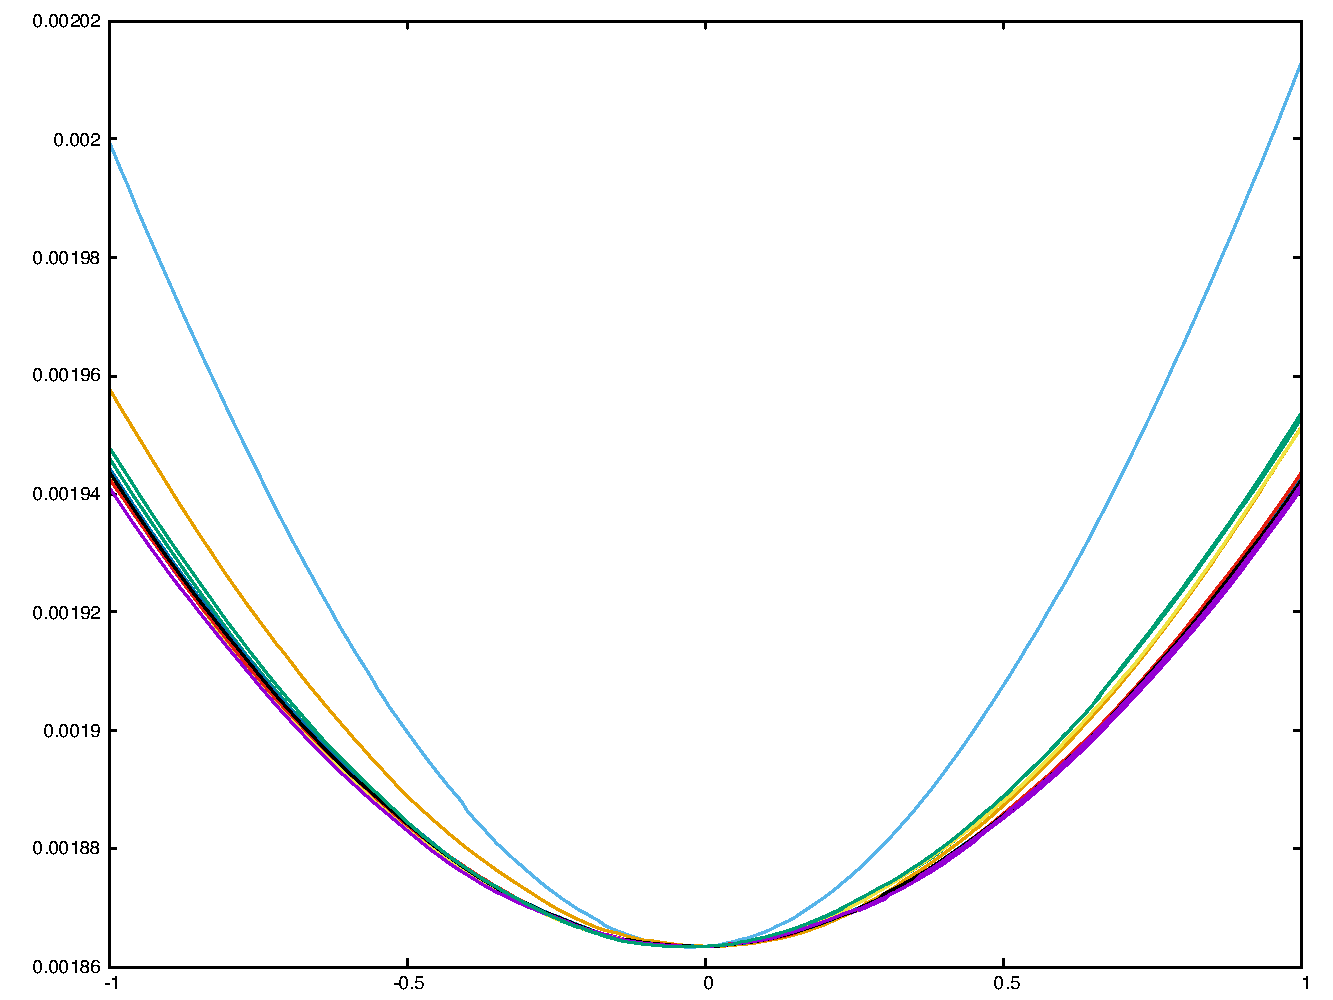
\includegraphics[width=\linewidth]{fig/ajherr/t/S_mae.pdf}
	\caption{S}
\end{subfigure}\\
\end{figure}

\paragraph{Observations} Firstly, it can be seen that the histogram comparison error metric $e_{\chi}$ is indeed an error metric for the registration. But no improvement compared to the mean absolute error can be seen. For large transformations, $e_{\chi}$ diverges, which is expected because the points $q$ are far away from the parallelogram lattice of $P$, making the histogram comparison results meaningless. For the scale M, the qualities of the error metrics are about the same. On scale $S$, the metric $e_{\chi}$ degenerates, but the mean absolute error remains more stable.


\subsection{Different view-points}
Here the resolutions are the same, but $P$ and $Q$ are projections from different view-points, and the overlap is lower.

\begin{figure}[H]
\begin{subfigure}{.33\textwidth}
	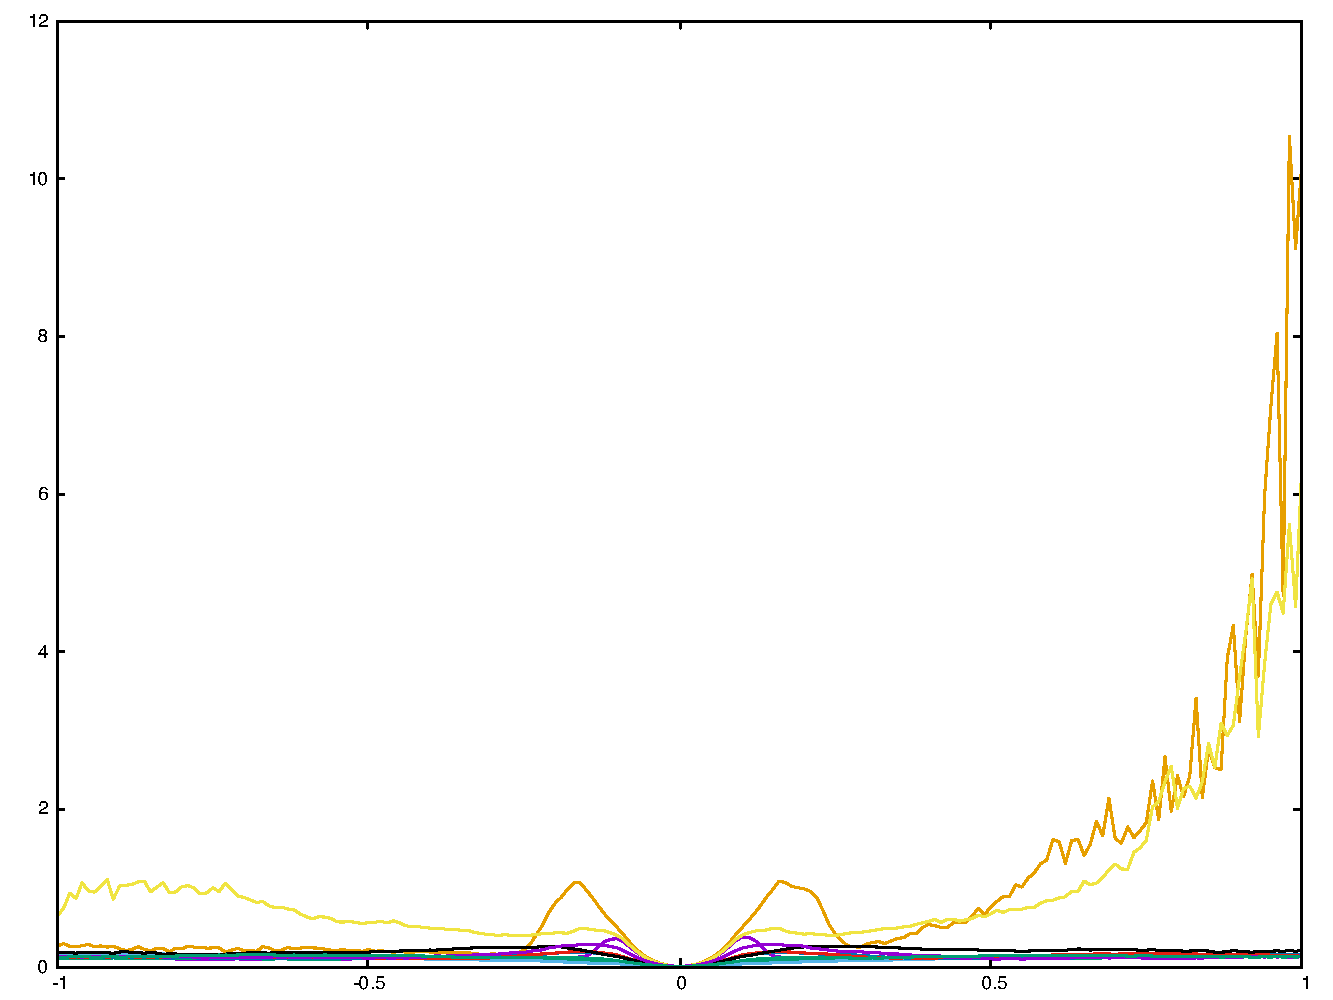
\includegraphics[width=\linewidth]{fig/ajherr/t2/L_chi.pdf}
\end{subfigure}%
\begin{subfigure}{.33\textwidth}
	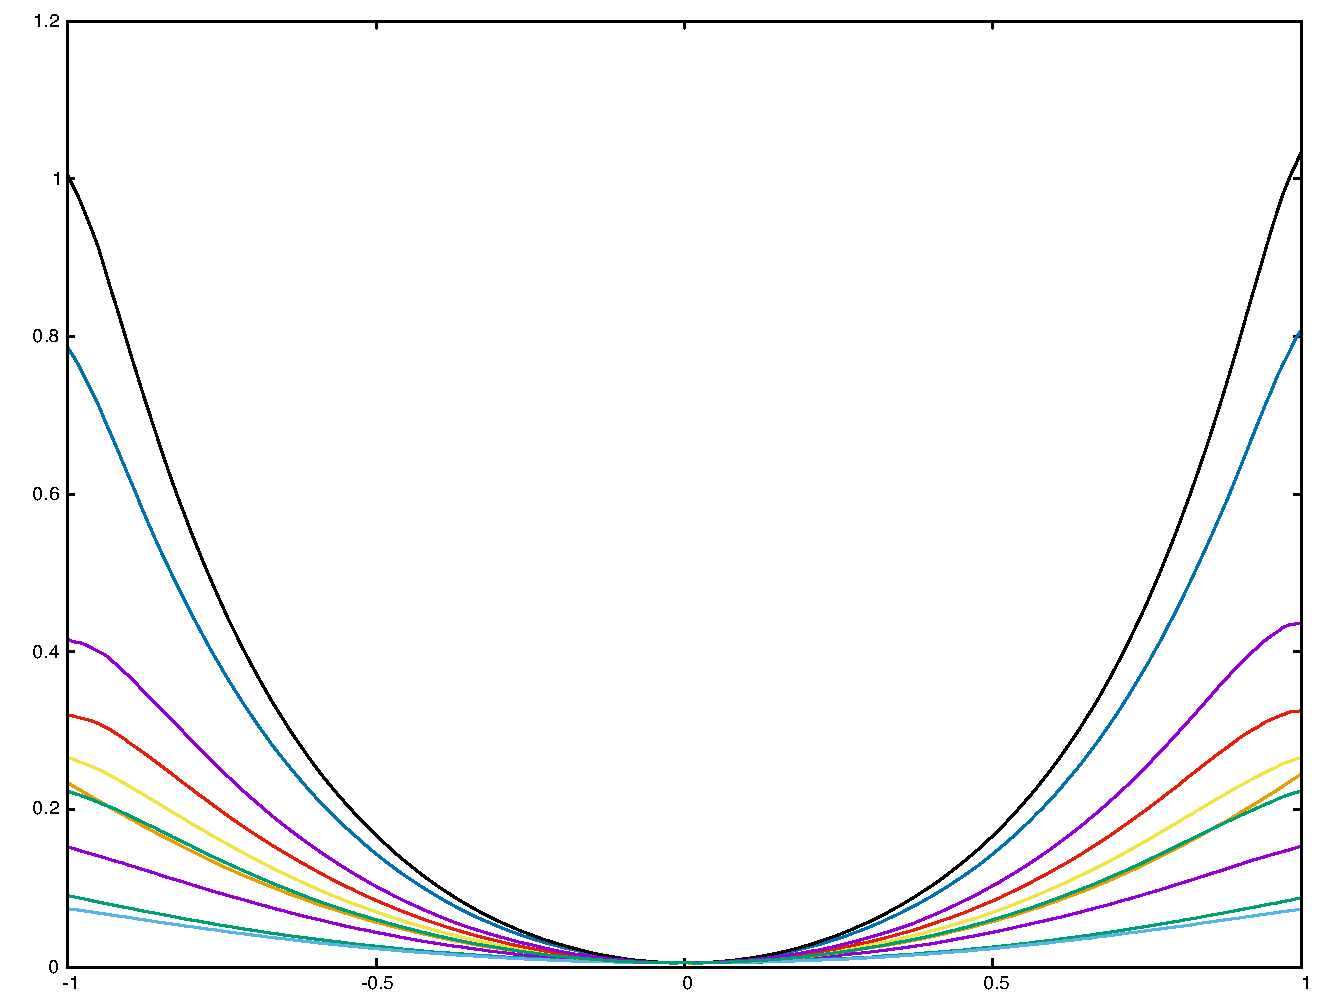
\includegraphics[width=\linewidth]{fig/ajherr/t2/M_chi.pdf}
\end{subfigure}&
\begin{subfigure}{.33\textwidth}
	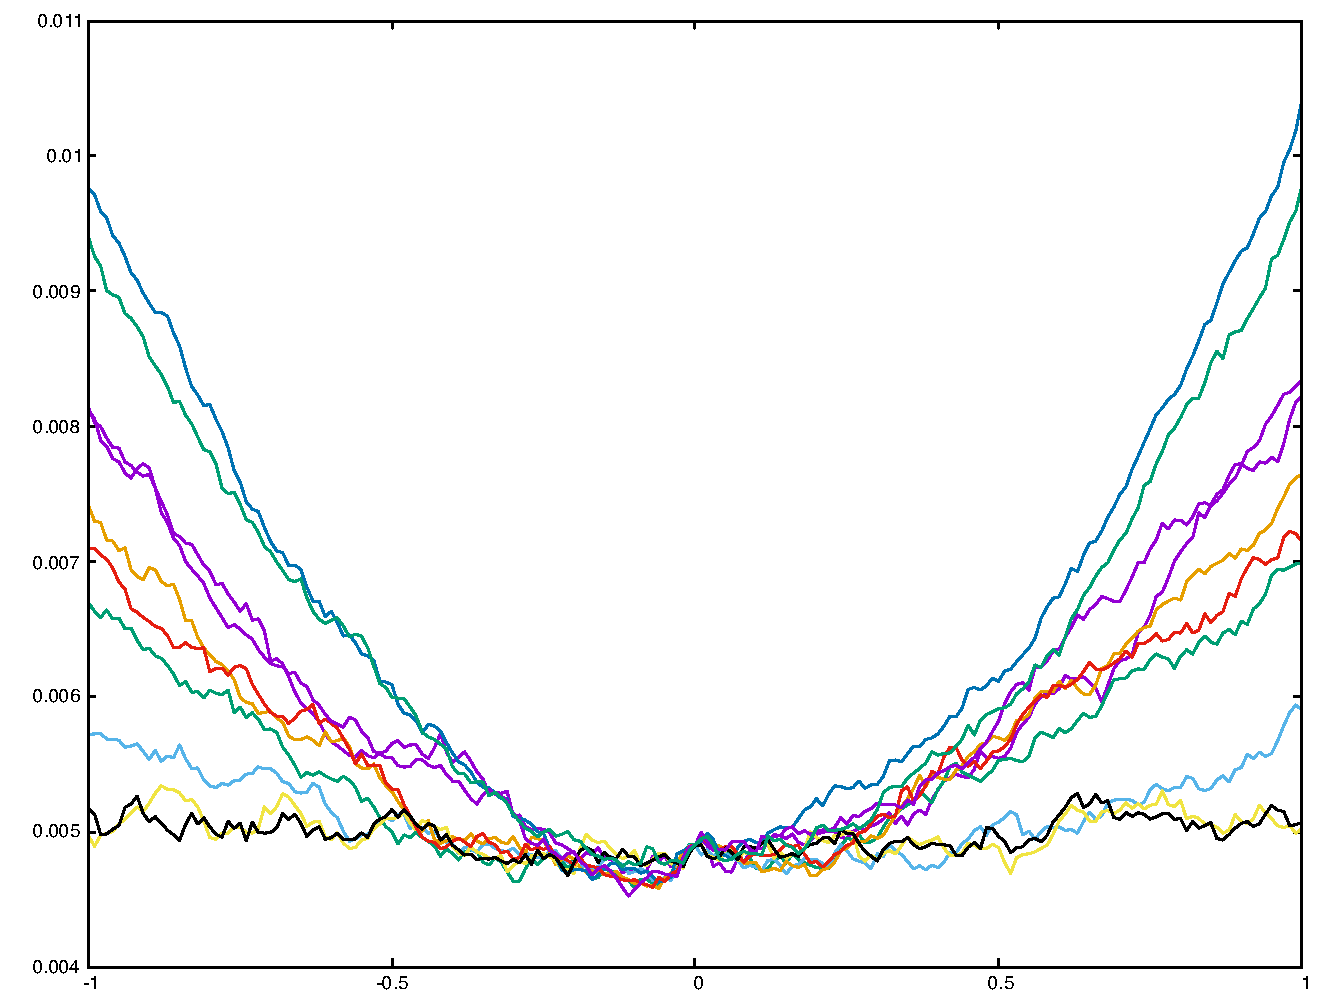
\includegraphics[width=\linewidth]{fig/ajherr/t2/S_chi.pdf}
\end{subfigure}\\
\begin{subfigure}{.33\textwidth}
	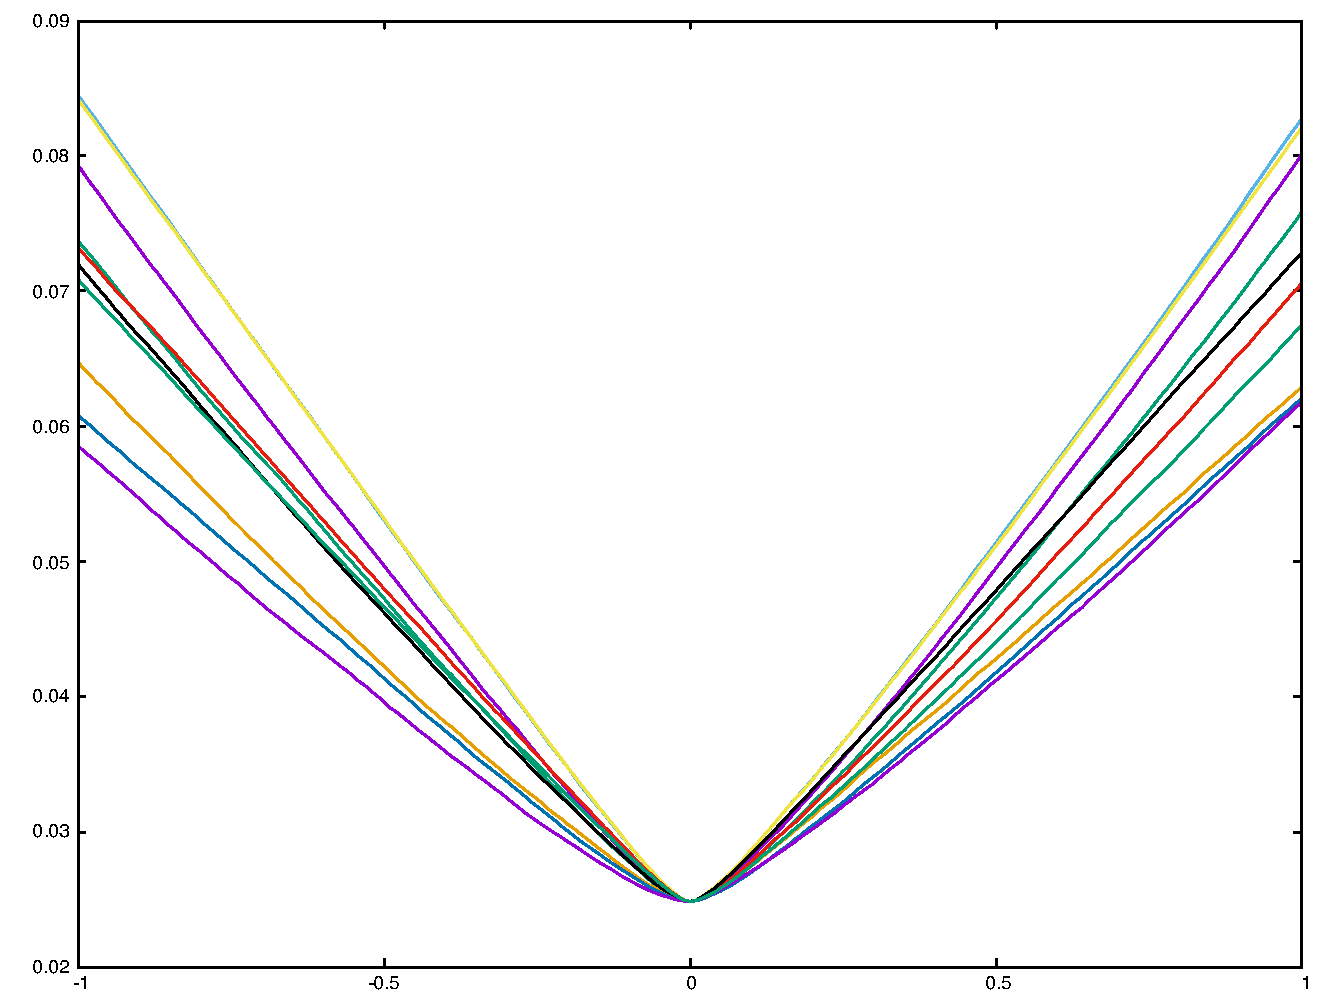
\includegraphics[width=\linewidth]{fig/ajherr/t2/L_mae.pdf}
	\caption{L}
\end{subfigure}%
\begin{subfigure}{.33\textwidth}
	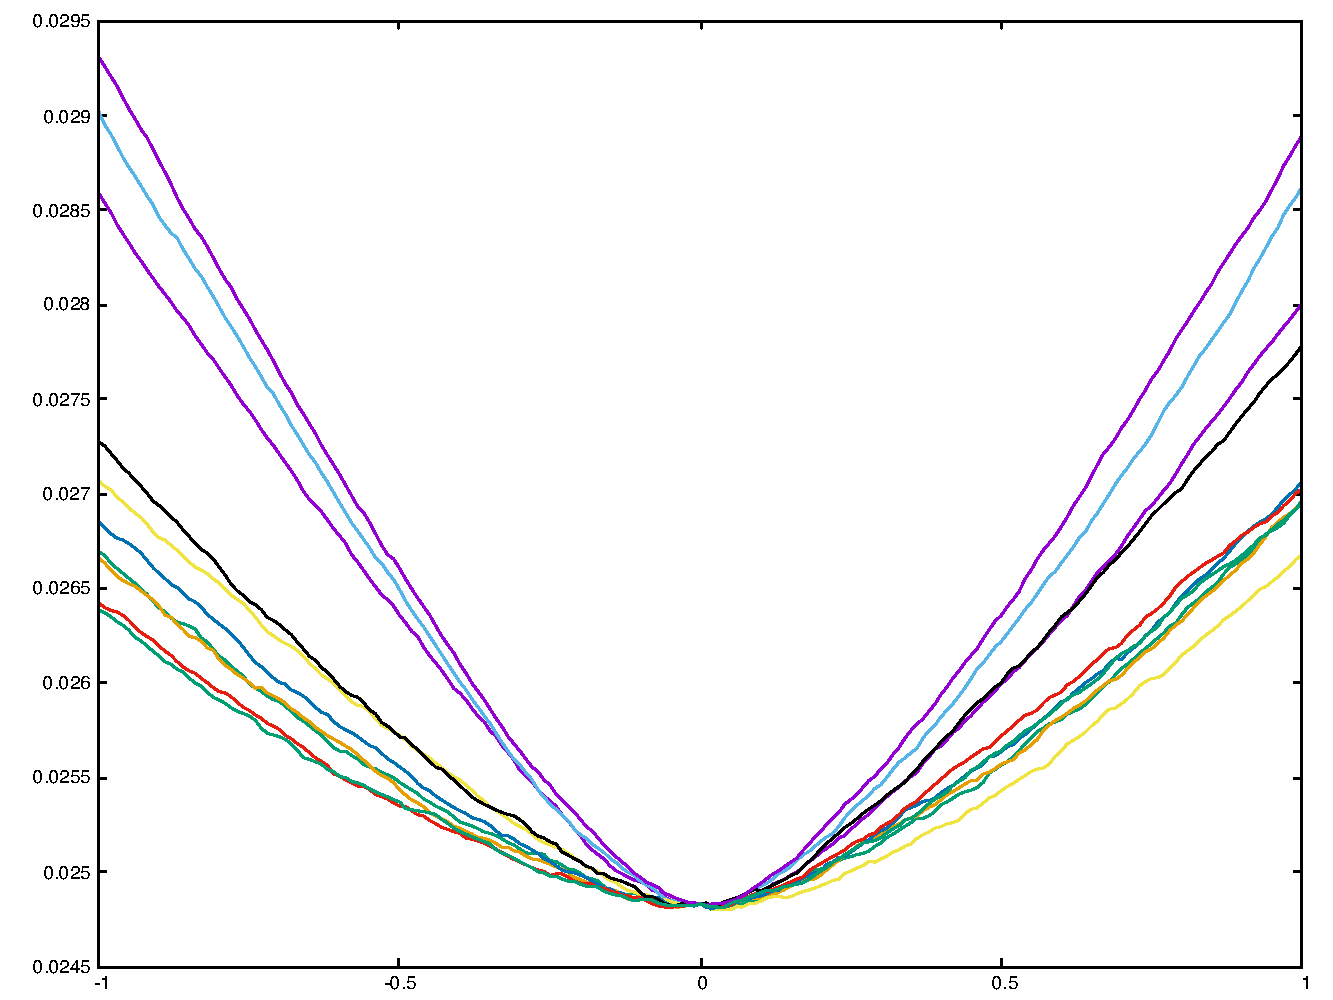
\includegraphics[width=\linewidth]{fig/ajherr/t2/M_mae.pdf}
	\caption{M}
\end{subfigure}&
\begin{subfigure}{.33\textwidth}
	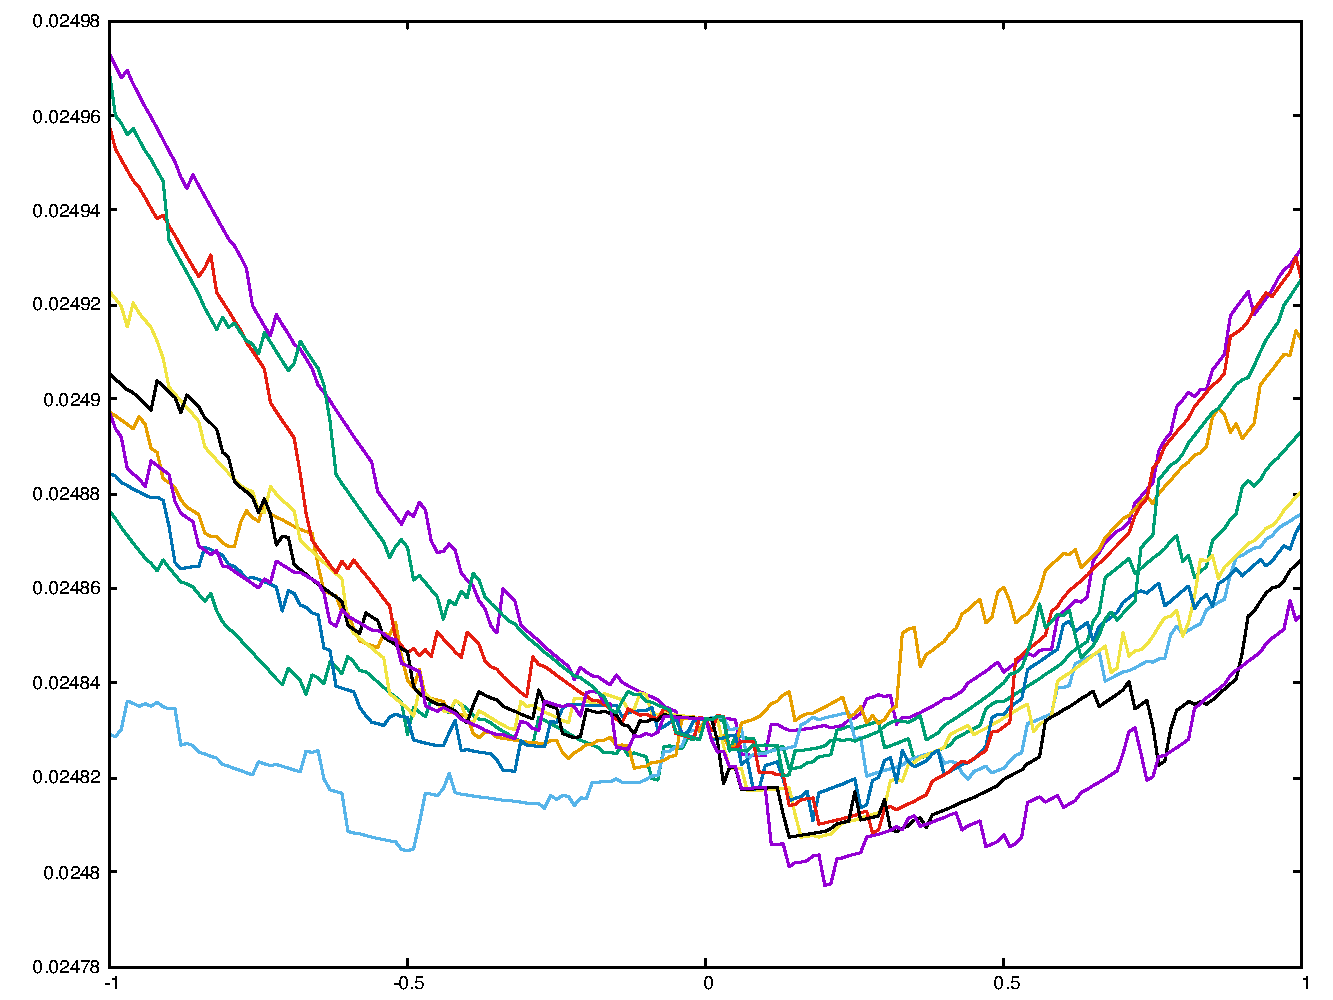
\includegraphics[width=\linewidth]{fig/ajherr/t2/S_mae.pdf}
	\caption{S}
\end{subfigure}\\
\end{figure}

\paragraph{Observations} The results are similar than before. But on the S scale, both $e_{\chi}$ and the mean absolute error degenerate, as there is a lower number of point correspondences. On this example, $e_{\chi}$ appears to remain slightly more stable.


\FloatBarrier


\subsection{Different resolutions}
Here $P$ has a much lower resolution than $Q$. Again the scale is seen on the close-up view on figure \ref{fig:t3_scale}.

\begin{figure}[h]
\center
{
\setlength{\fboxsep}{0pt}%
\setlength{\fboxrule}{0.5pt}%
\fbox{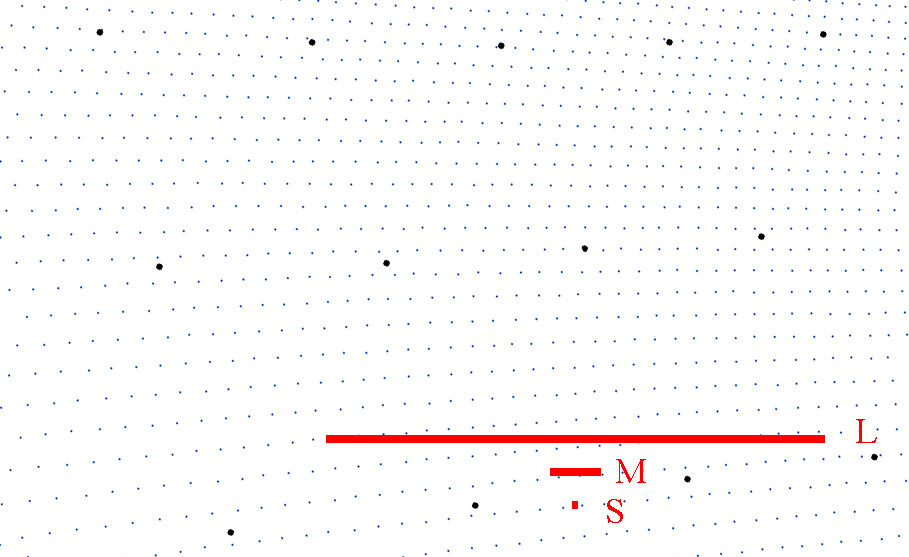
\includegraphics[width=0.4\textwidth]{fig/t3_scale.png}}
}
\label{fig:t3_scale}
\caption{Close-up view with scale}
\end{figure}


\begin{figure}[H]
\begin{subfigure}{.33\textwidth}
	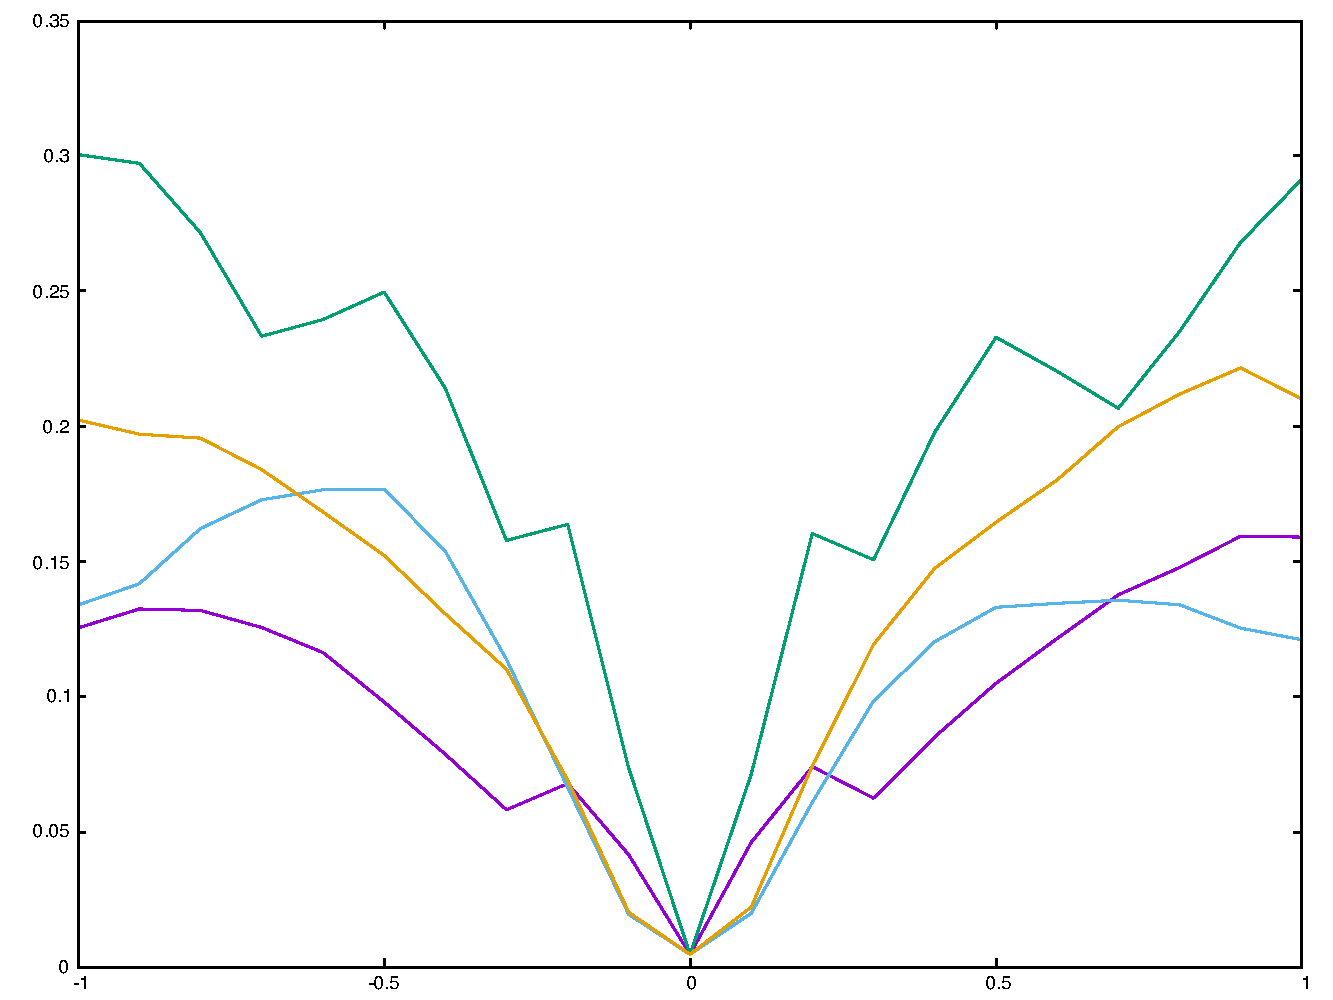
\includegraphics[width=\linewidth]{fig/ajherr/t3/L_chi.pdf}
\end{subfigure}%
\begin{subfigure}{.33\textwidth}
	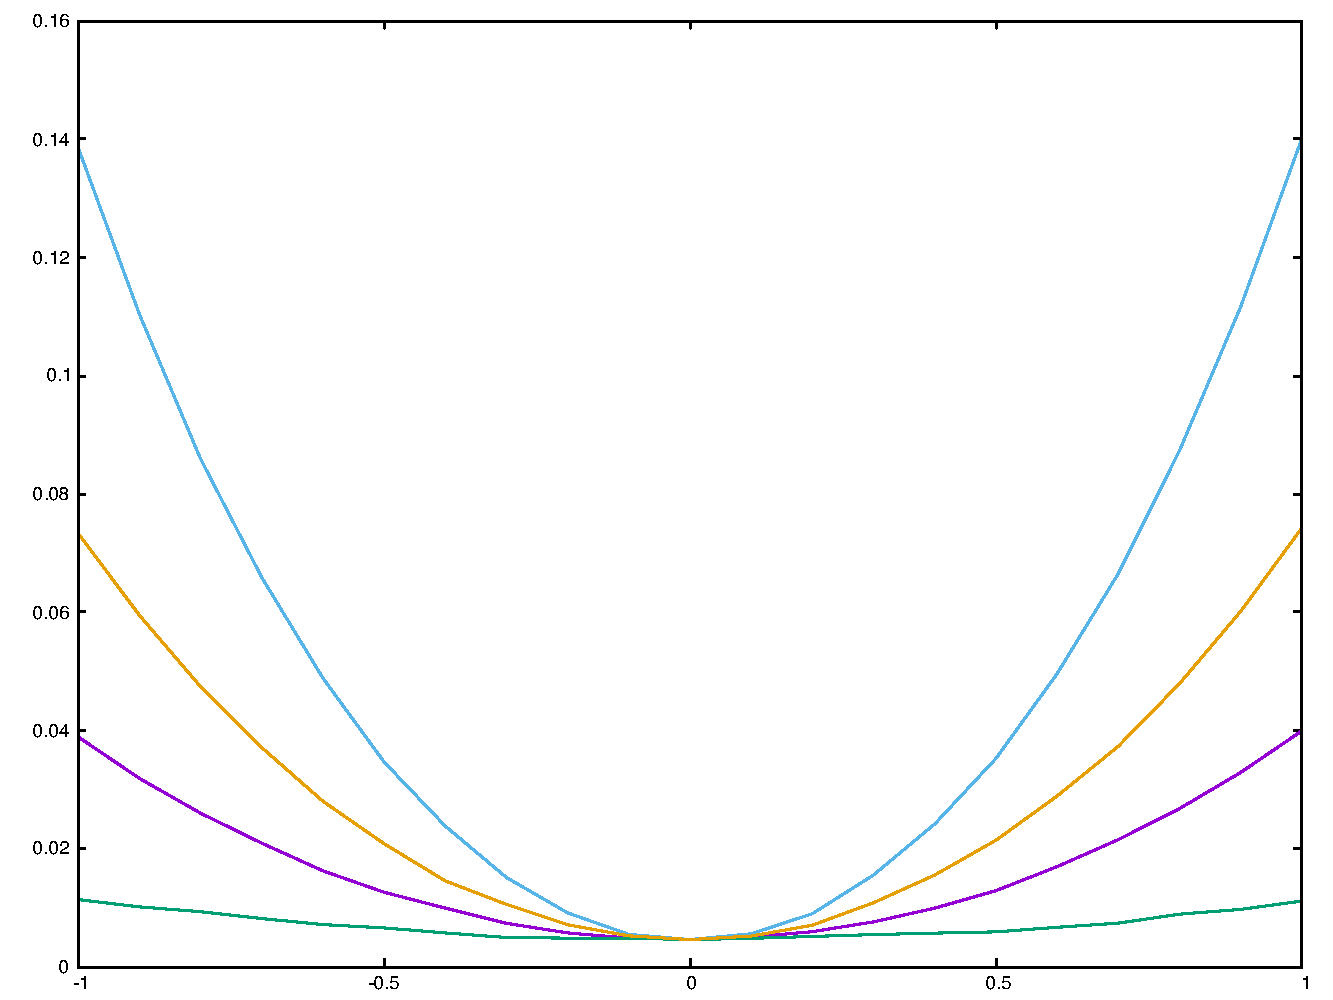
\includegraphics[width=\linewidth]{fig/ajherr/t3/M_chi.pdf}
\end{subfigure}&
\begin{subfigure}{.33\textwidth}
	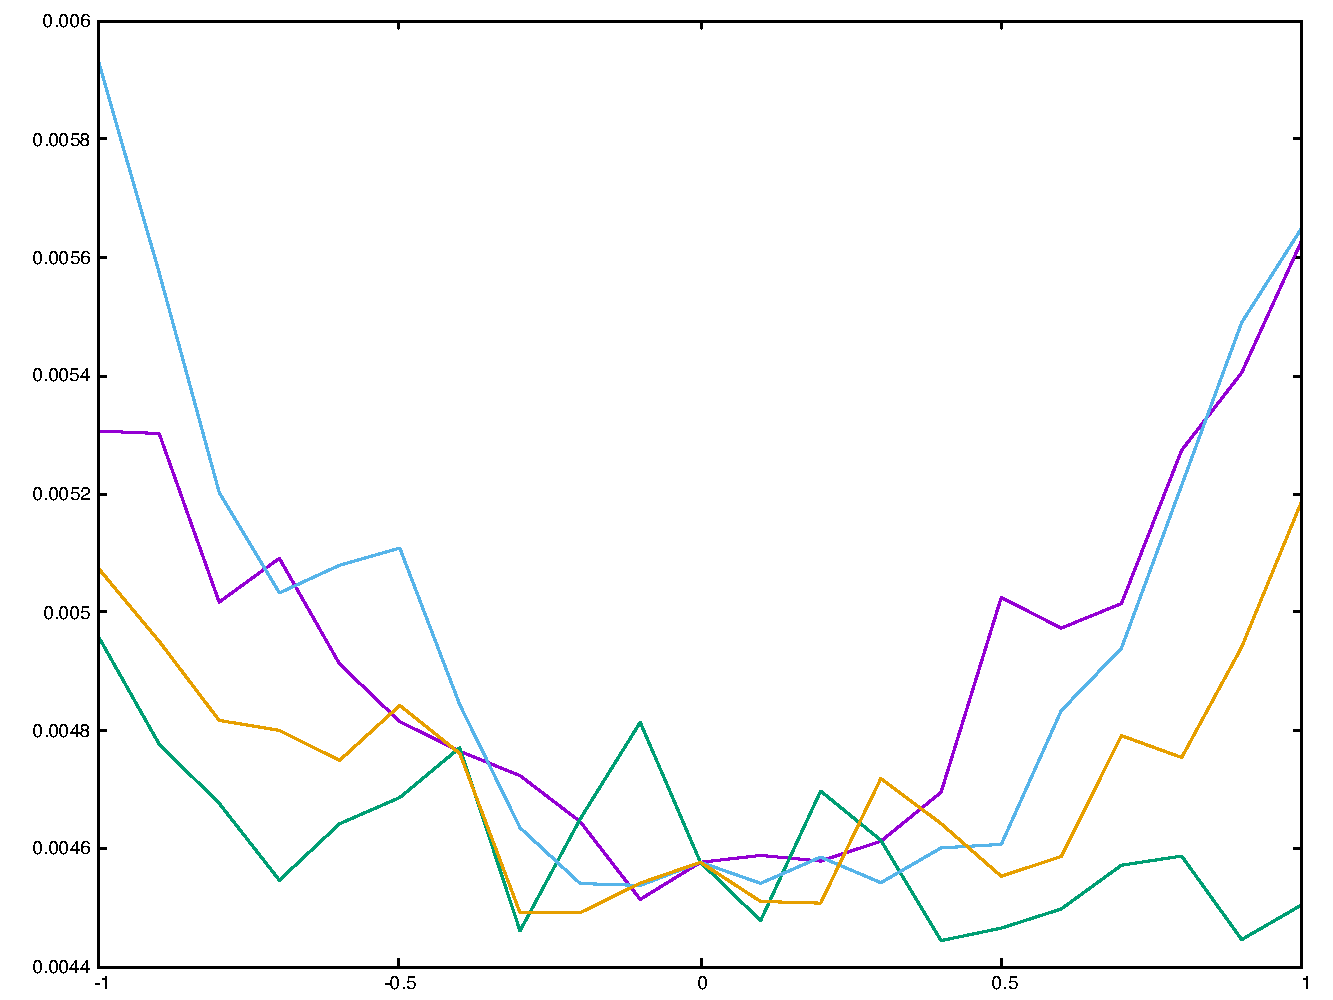
\includegraphics[width=\linewidth]{fig/ajherr/t3/S_chi.pdf}
\end{subfigure}\\
\begin{subfigure}{.33\textwidth}
	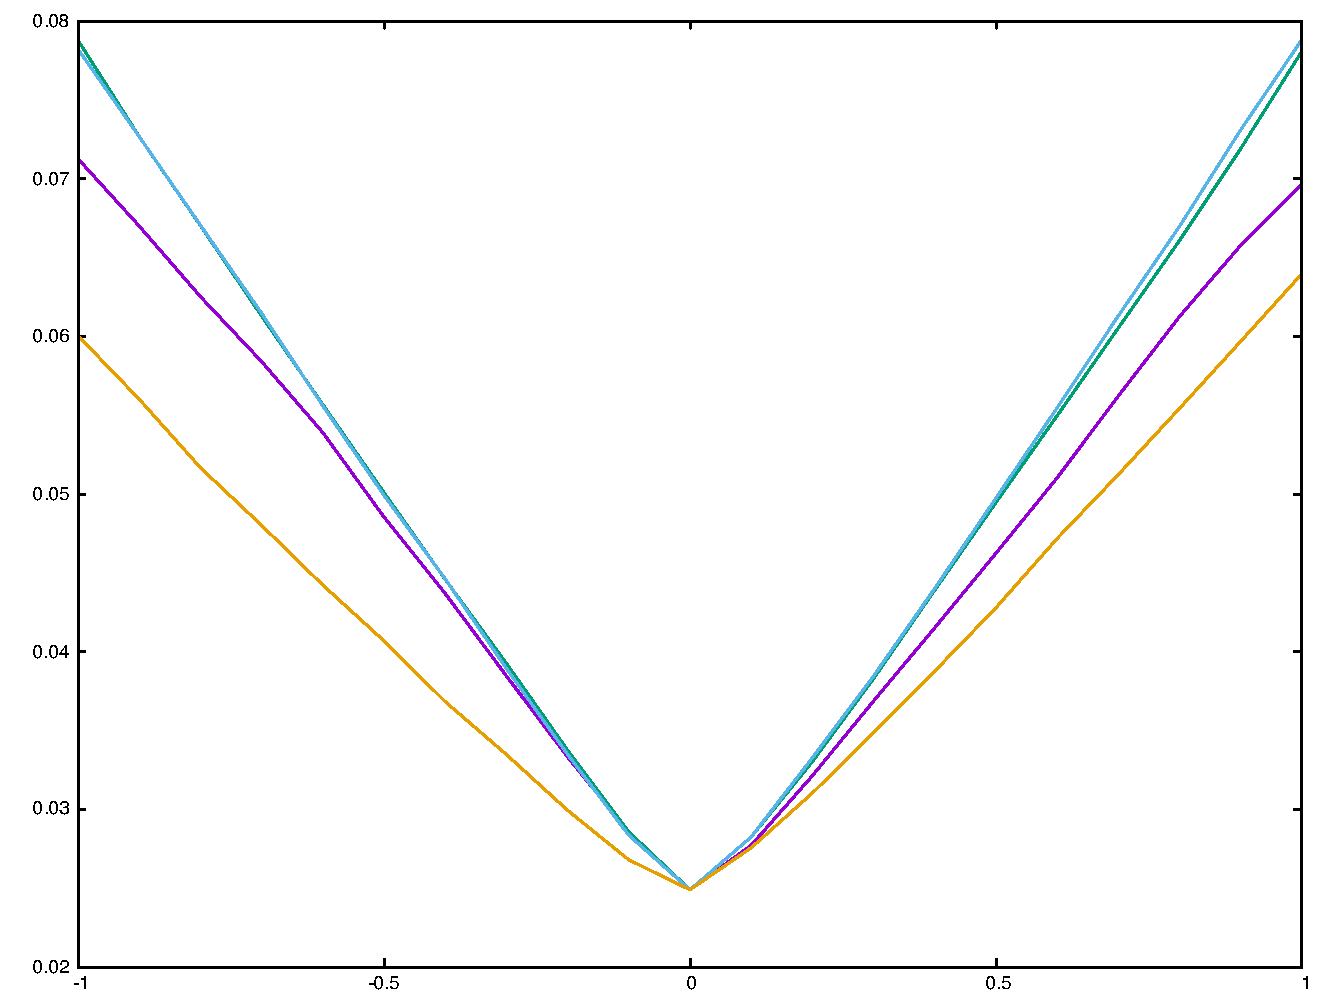
\includegraphics[width=\linewidth]{fig/ajherr/t3/L_mae.pdf}
	\caption{L}
\end{subfigure}%
\begin{subfigure}{.33\textwidth}
	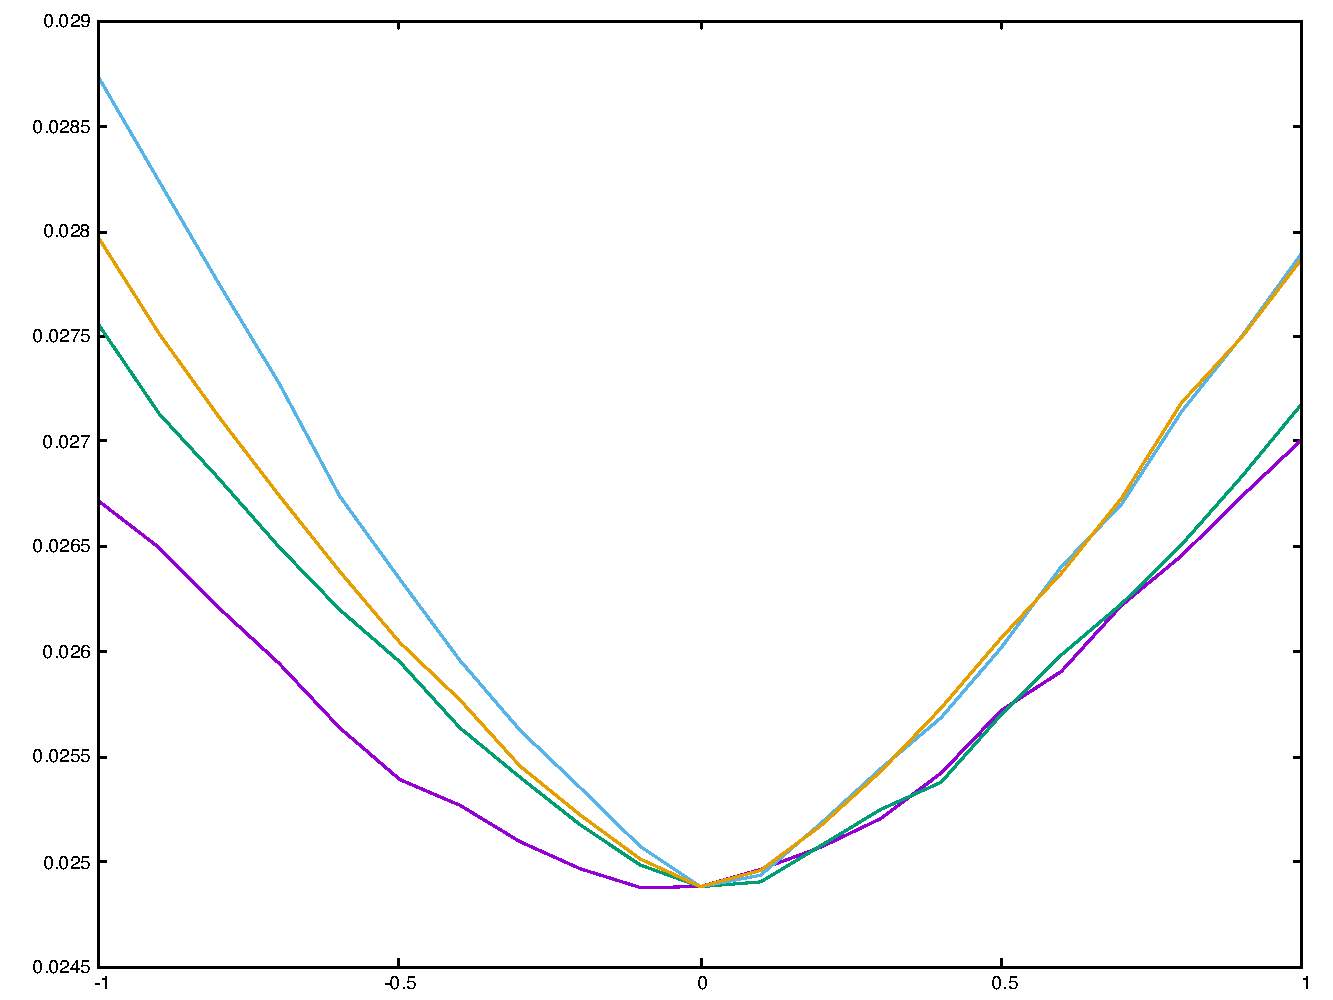
\includegraphics[width=\linewidth]{fig/ajherr/t3/M_mae.pdf}
	\caption{M}
\end{subfigure}&
\begin{subfigure}{.33\textwidth}
	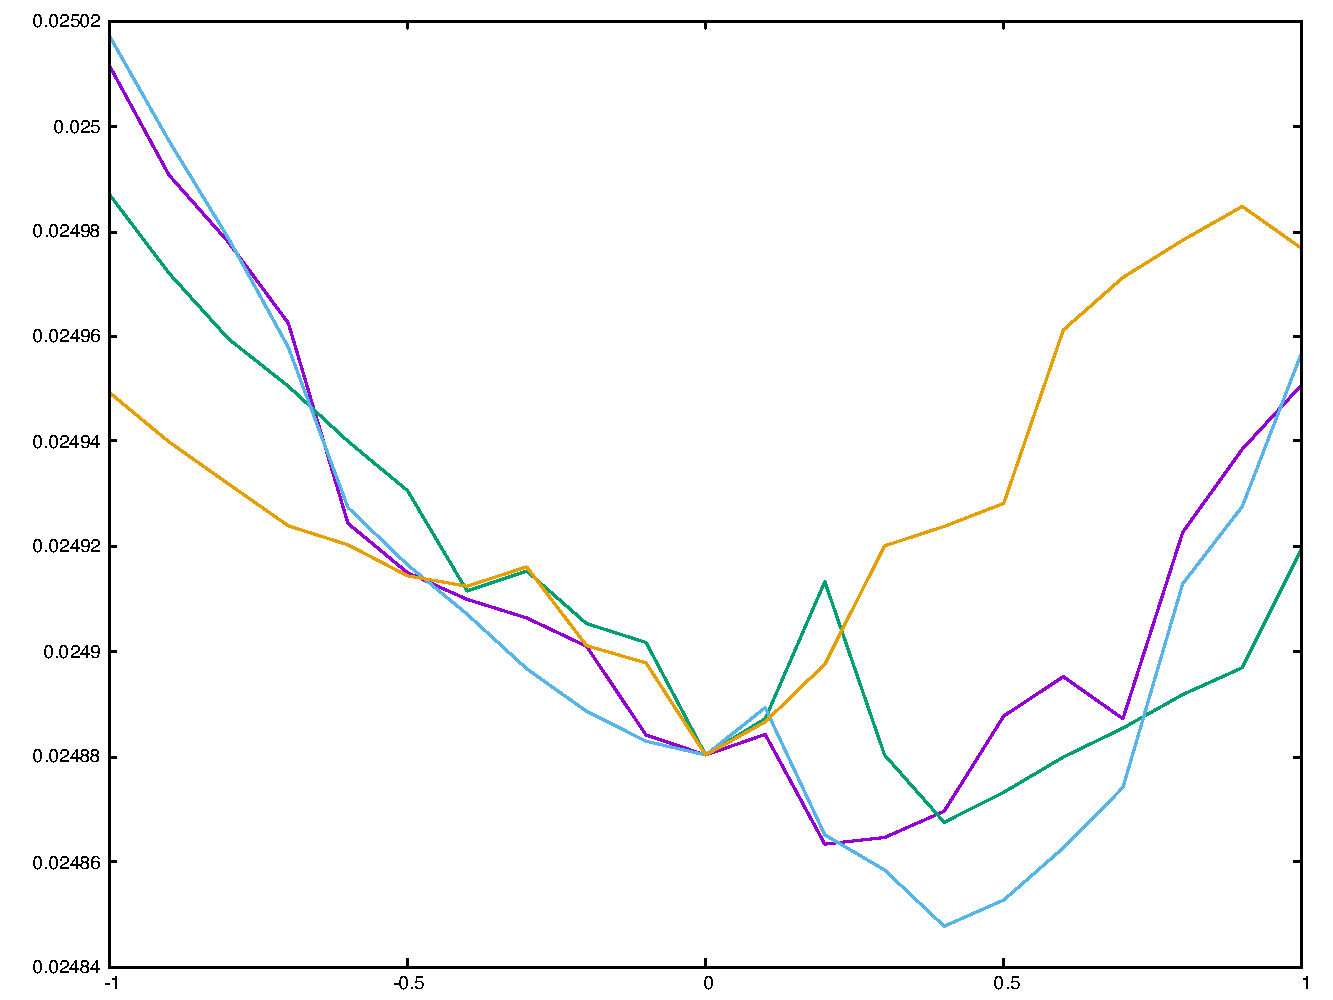
\includegraphics[width=\linewidth]{fig/ajherr/t3/S_mae.pdf}
	\caption{S}
\end{subfigure}\\
\end{figure}


\paragraph{Observations} To save time, these plots were recorded less precisely.\footnote{This means that the number of intermediary transformations $\matr{M'}$ at which the two error metrics are evaluated it lower, and there are fewer cross-section curves. The point clouds and their resolutions are the same. The plots are drawn as piecewise linear functions.} The results remain similar to before, no improvement of $e_{\chi}$ compared to the mean absolute error metric can be seen. 


\subsubsection{Translation only}
Here only the translational part of the transformation is applied.

\begin{figure}[H]
\begin{subfigure}{.33\textwidth}
	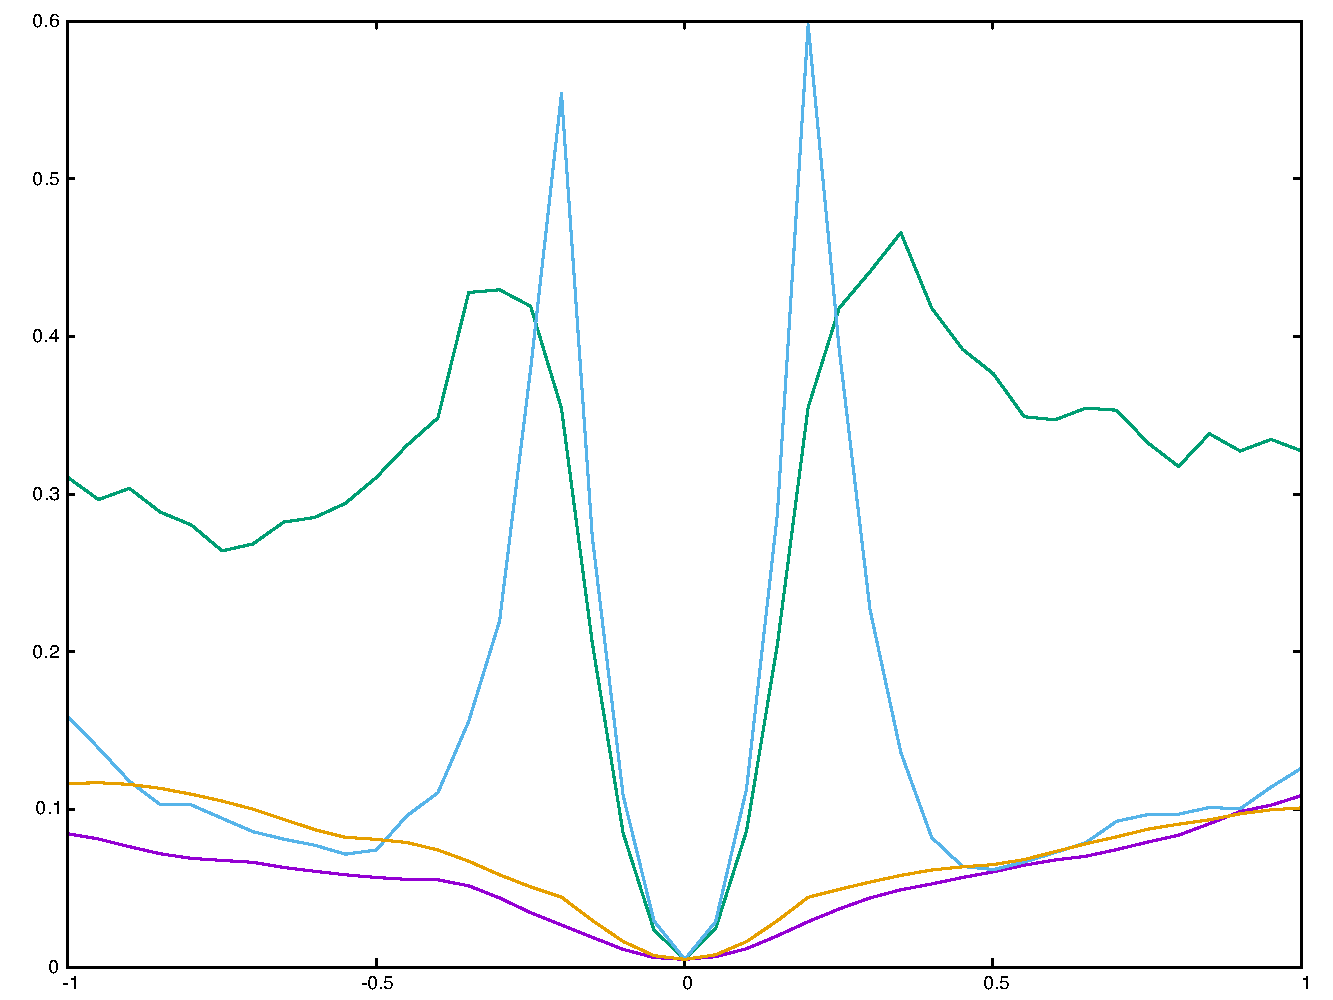
\includegraphics[width=\linewidth]{fig/ajherr/t3t/L_chi.pdf}
\end{subfigure}%
\begin{subfigure}{.33\textwidth}
	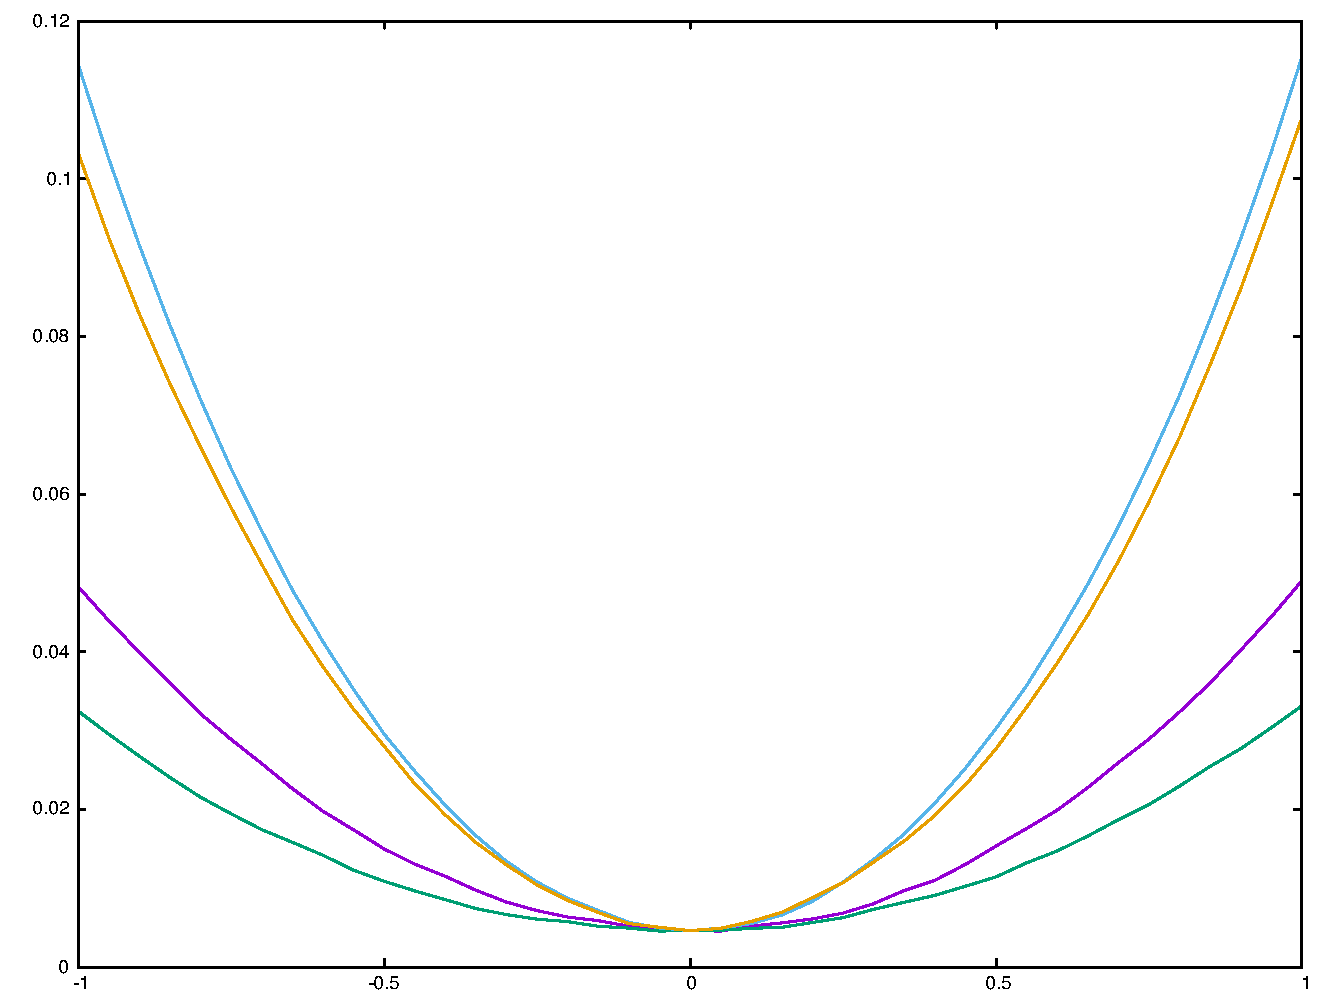
\includegraphics[width=\linewidth]{fig/ajherr/t3t/M_chi.pdf}
\end{subfigure}&
\begin{subfigure}{.33\textwidth}
	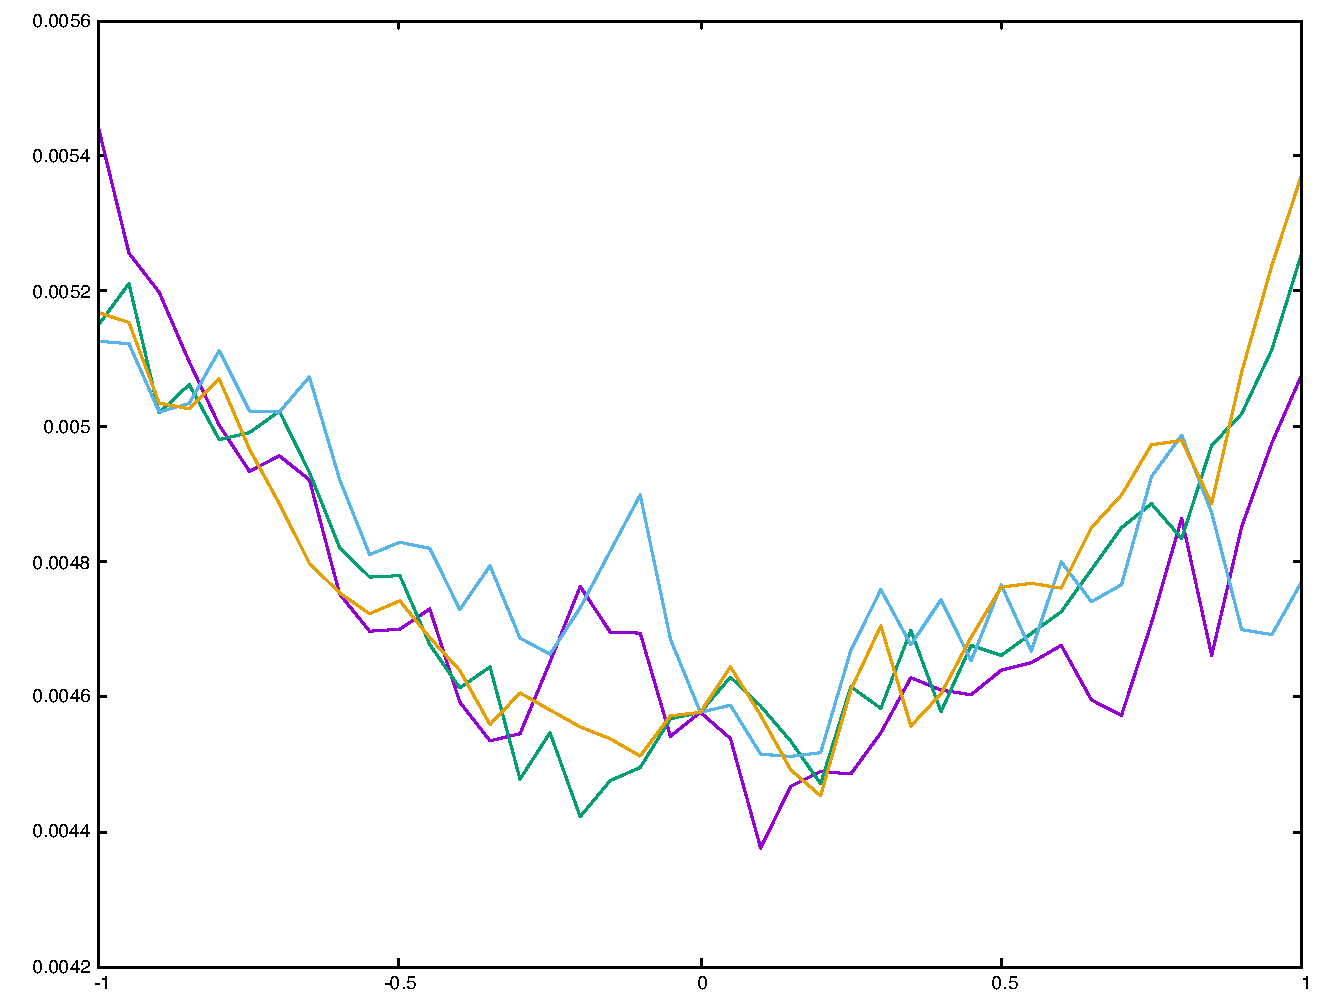
\includegraphics[width=\linewidth]{fig/ajherr/t3t/S_chi.pdf}
\end{subfigure}\\
\begin{subfigure}{.33\textwidth}
	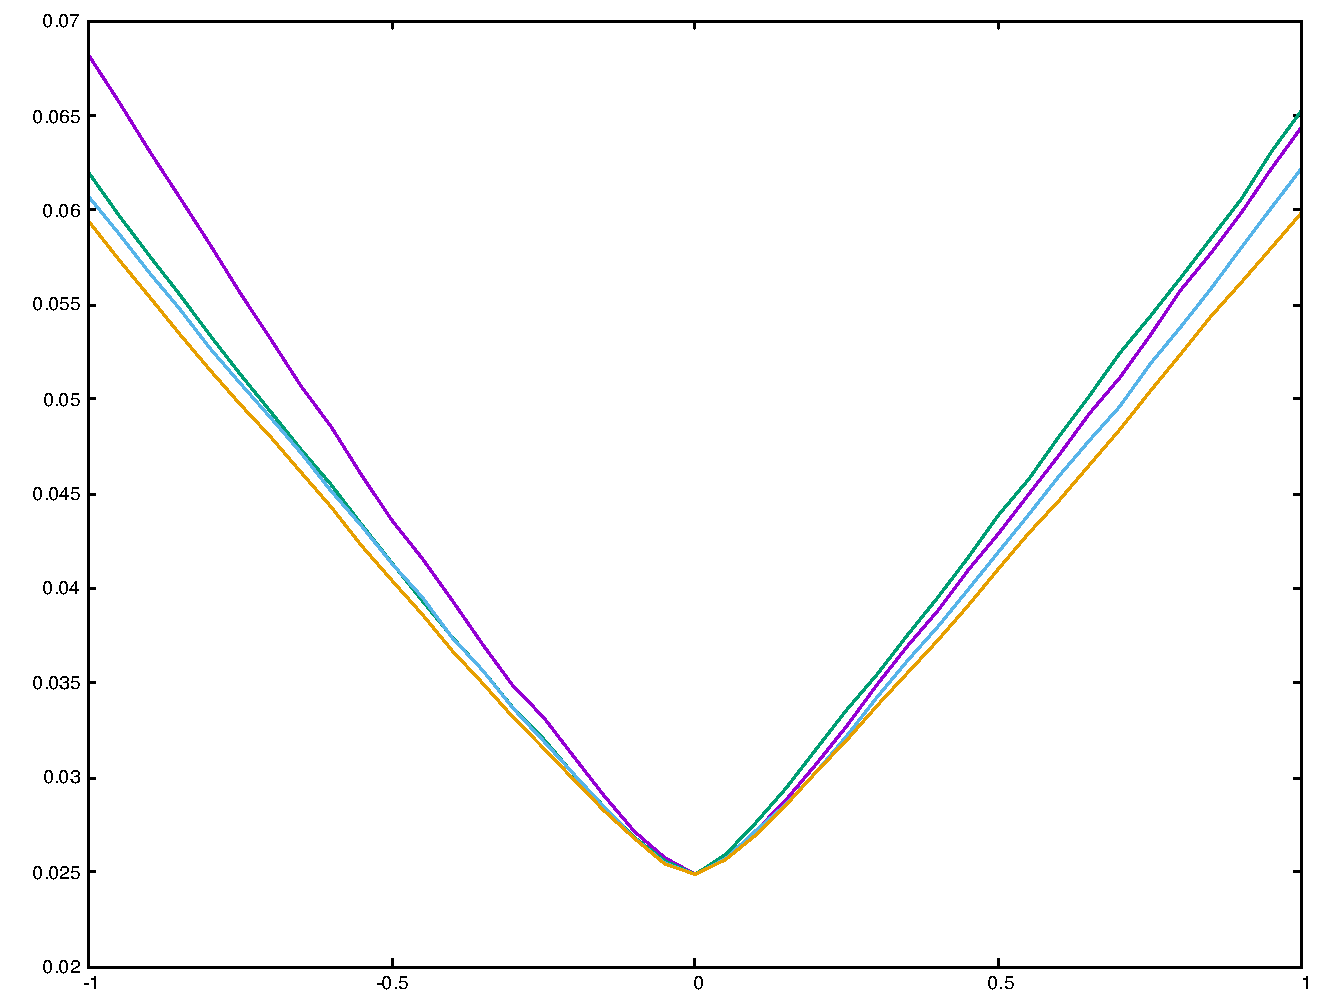
\includegraphics[width=\linewidth]{fig/ajherr/t3t/L_mae.pdf}
	\caption{L}
\end{subfigure}%
\begin{subfigure}{.33\textwidth}
	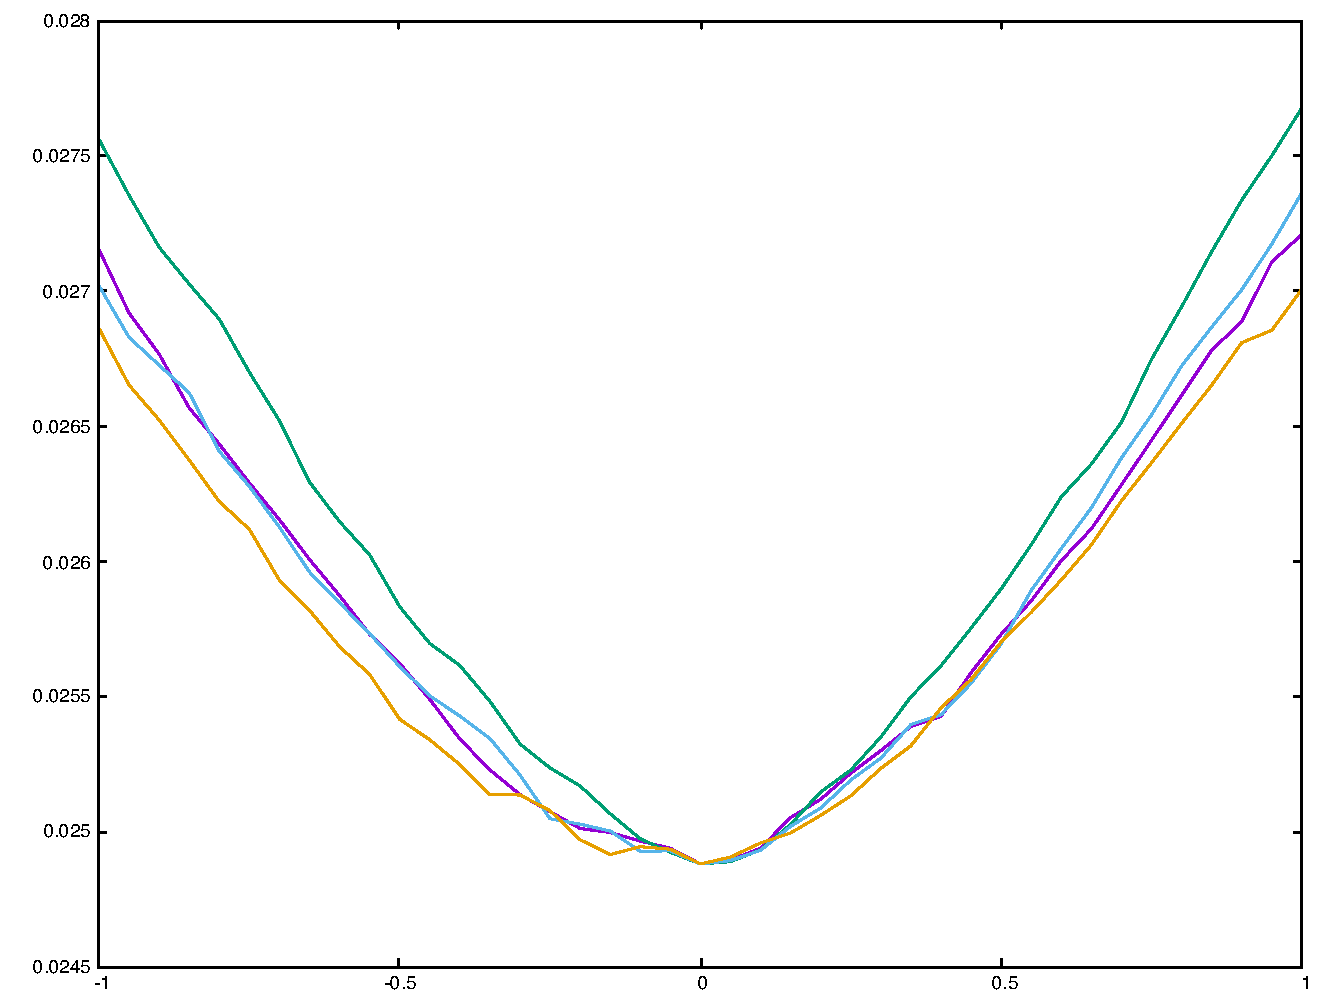
\includegraphics[width=\linewidth]{fig/ajherr/t3t/M_mae.pdf}
	\caption{M}
\end{subfigure}&
\begin{subfigure}{.33\textwidth}
	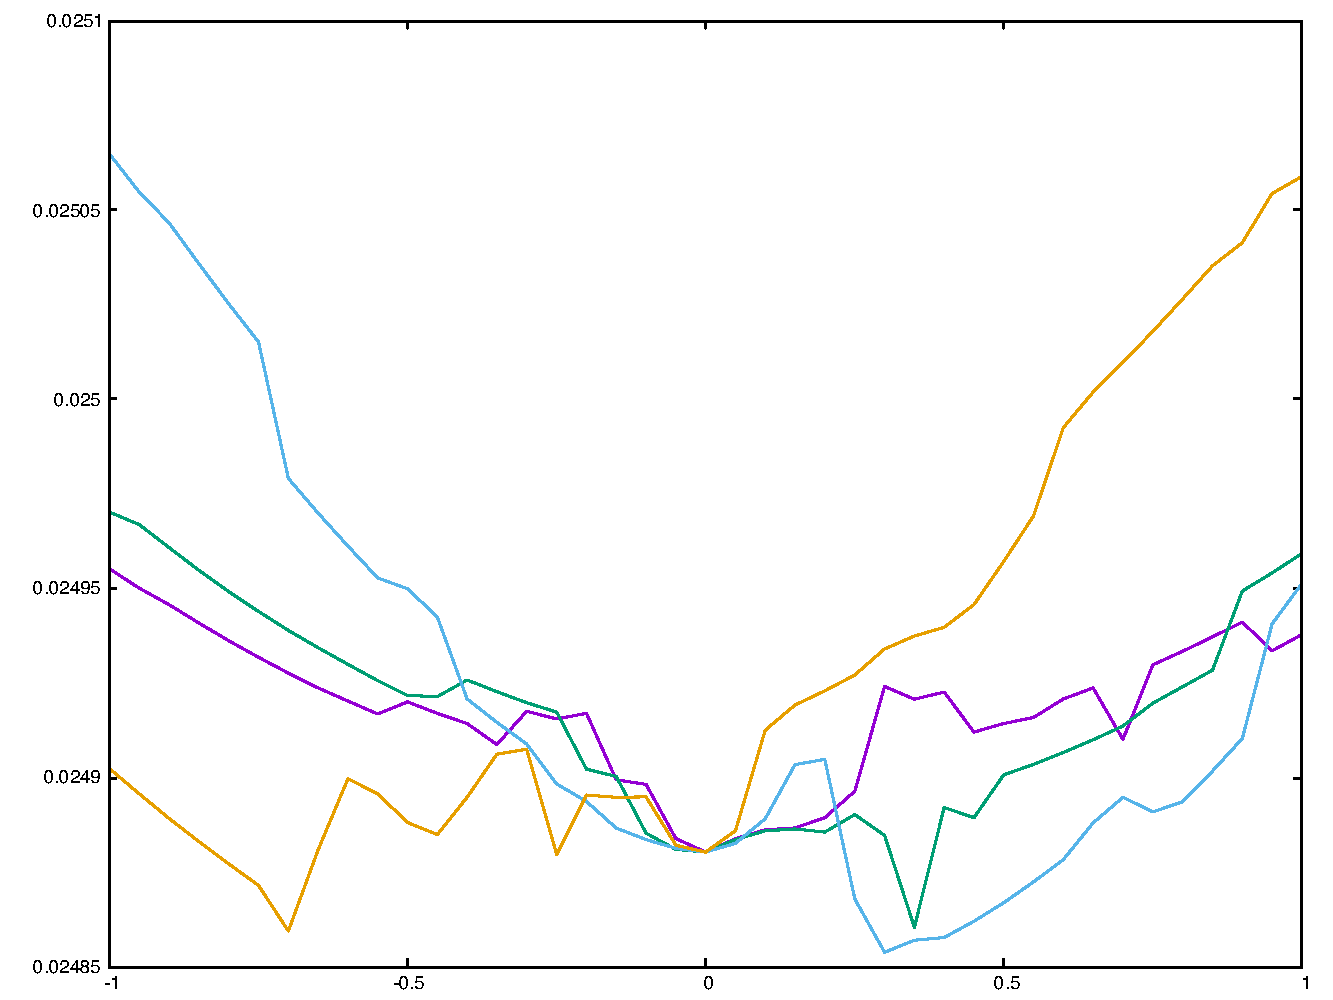
\includegraphics[width=\linewidth]{fig/ajherr/t3t/S_mae.pdf}
	\caption{S}
\end{subfigure}\\
\end{figure}

\paragraph{Observations} Again, no improvement of $e_{\chi}$ compared to mean absolute error.



\subsubsection{Rotation only}
Now only the rotational part is applied.


\begin{figure}[H]
\begin{subfigure}{.33\textwidth}
	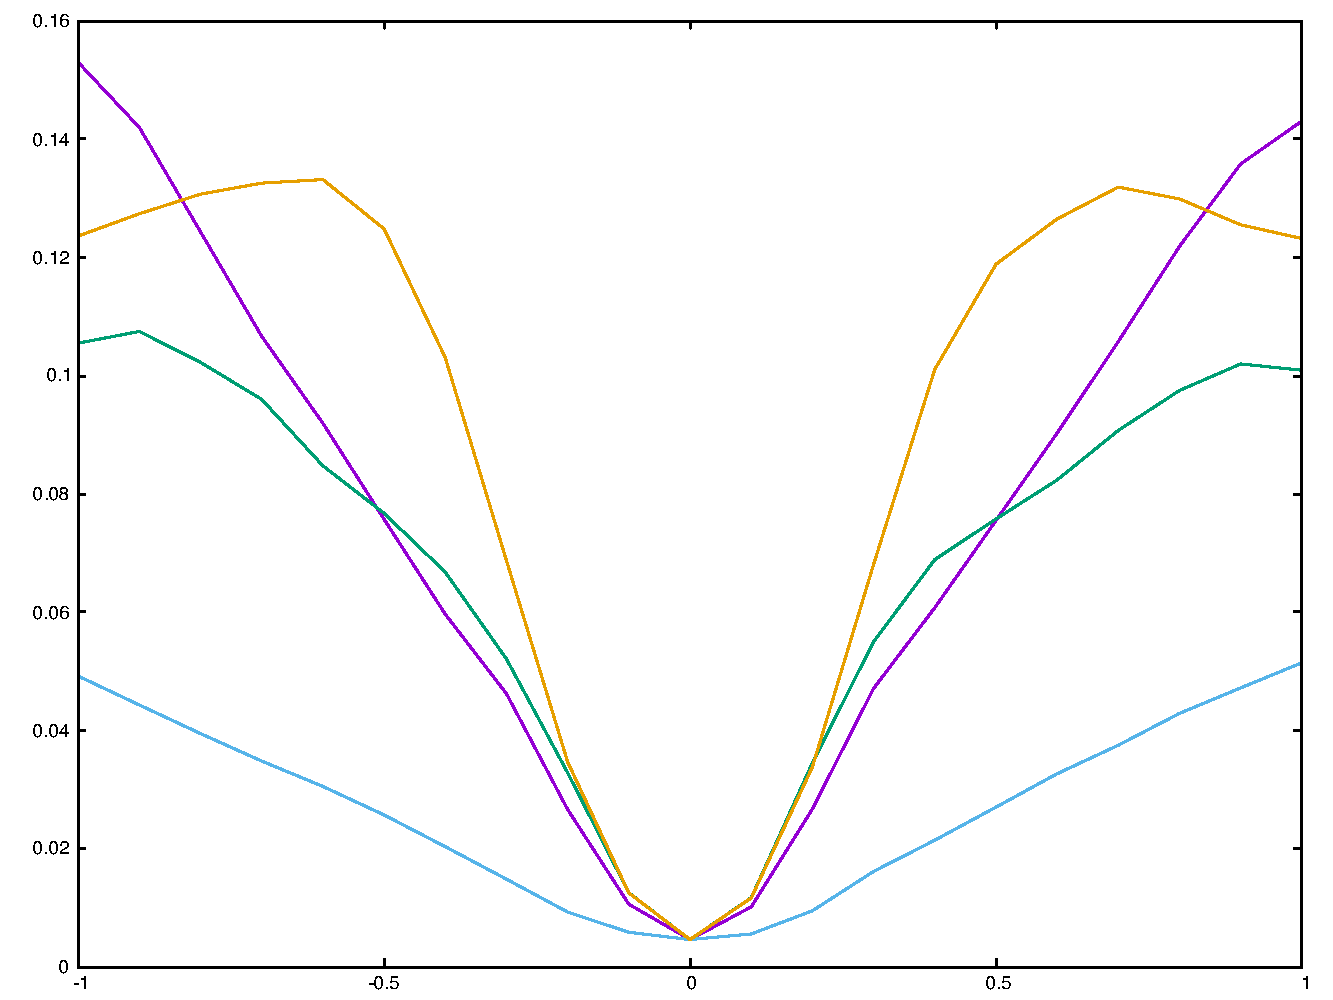
\includegraphics[width=\linewidth]{fig/ajherr/t3r/L_chi.pdf}
\end{subfigure}%
\begin{subfigure}{.33\textwidth}
	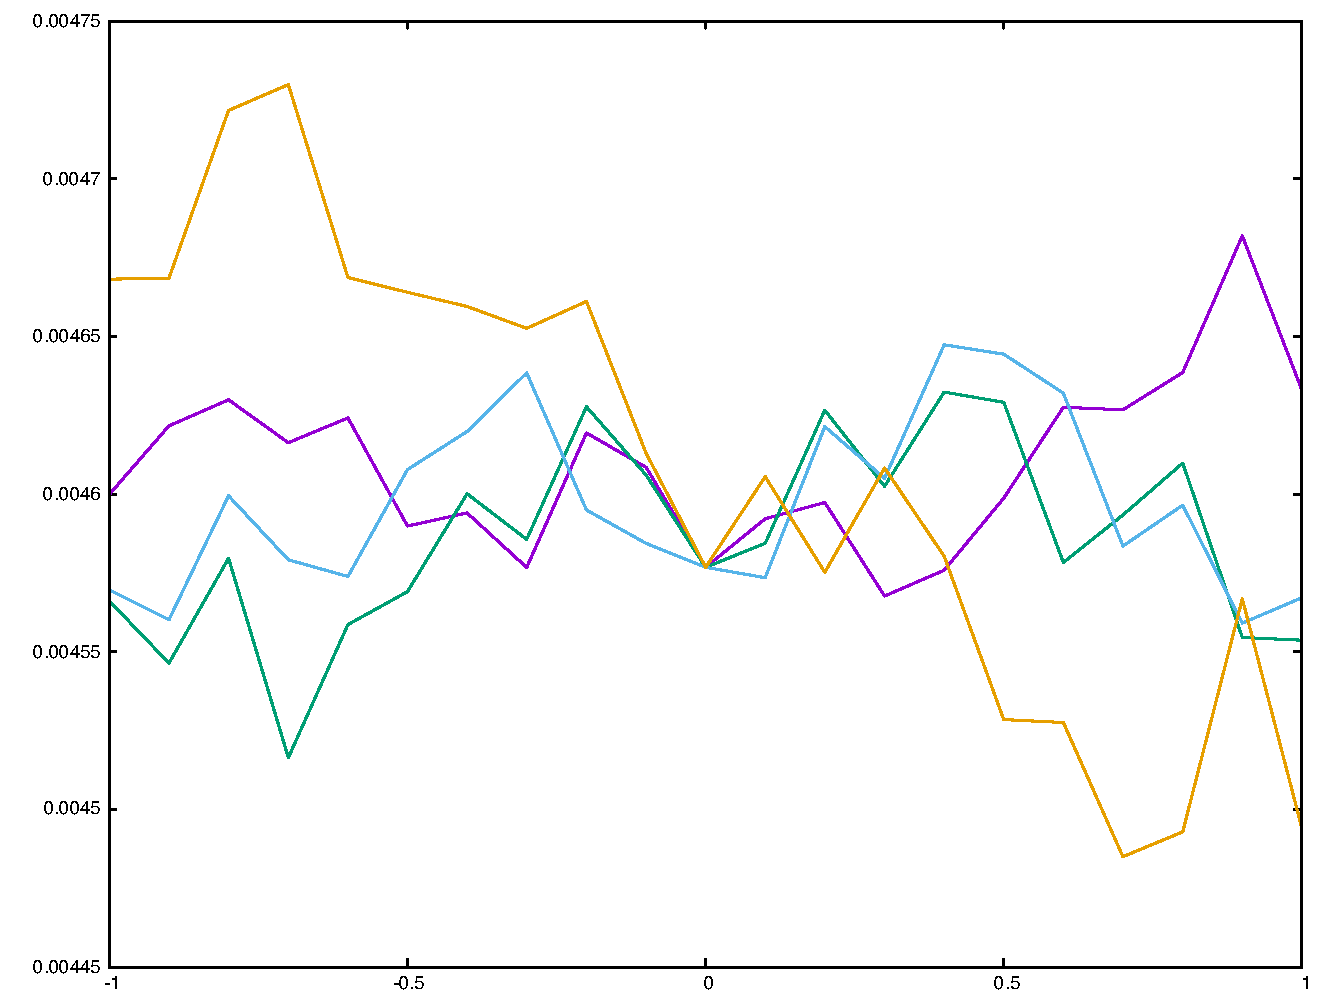
\includegraphics[width=\linewidth]{fig/ajherr/t3r/M_chi.pdf}
\end{subfigure}&
\begin{subfigure}{.33\textwidth}
	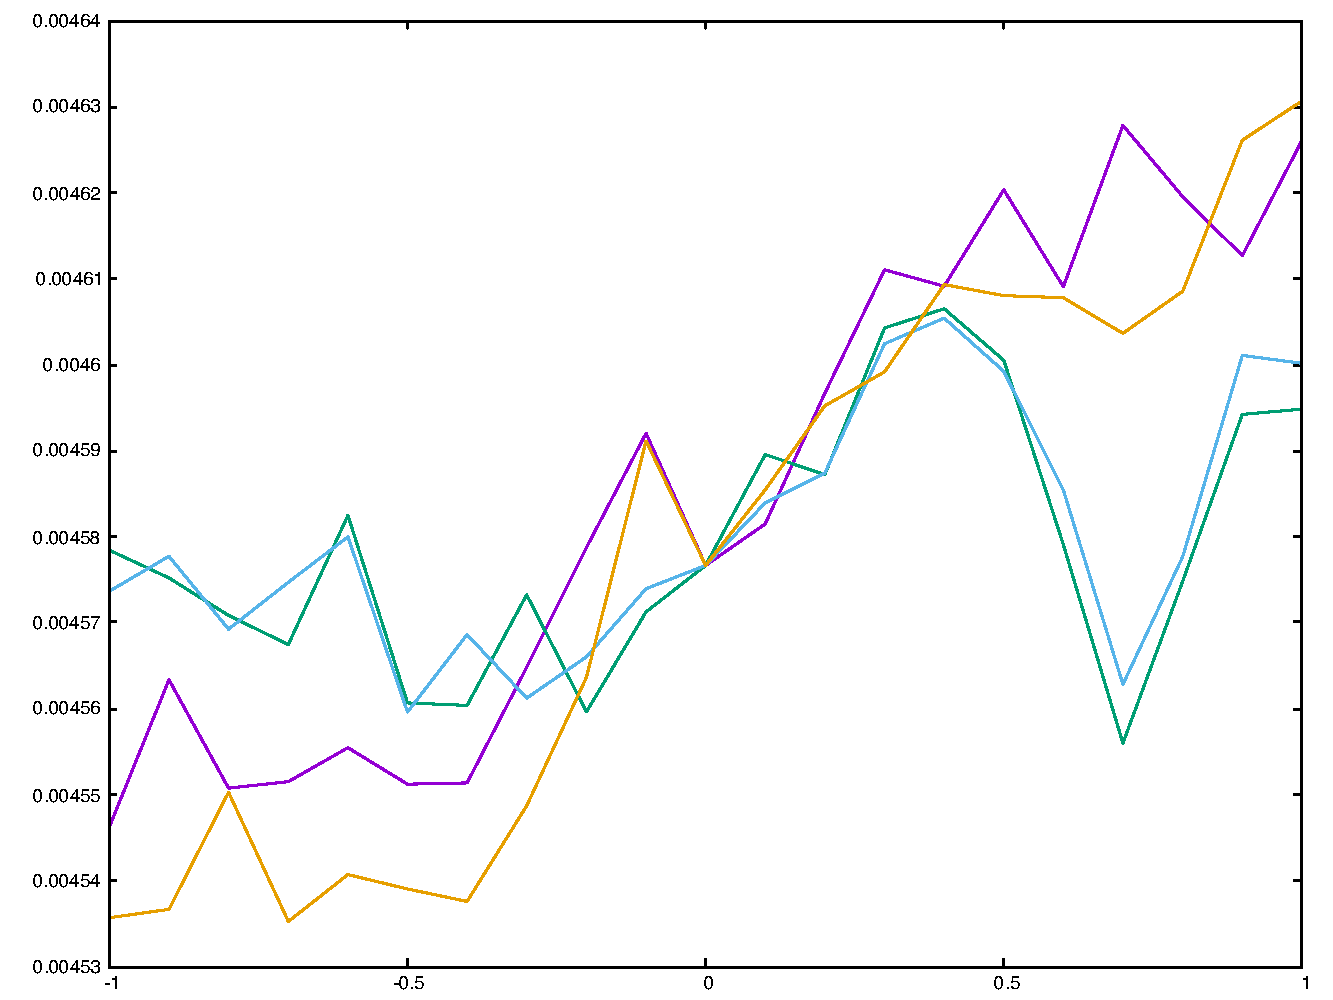
\includegraphics[width=\linewidth]{fig/ajherr/t3r/S_chi.pdf}
\end{subfigure}\\
\begin{subfigure}{.33\textwidth}
	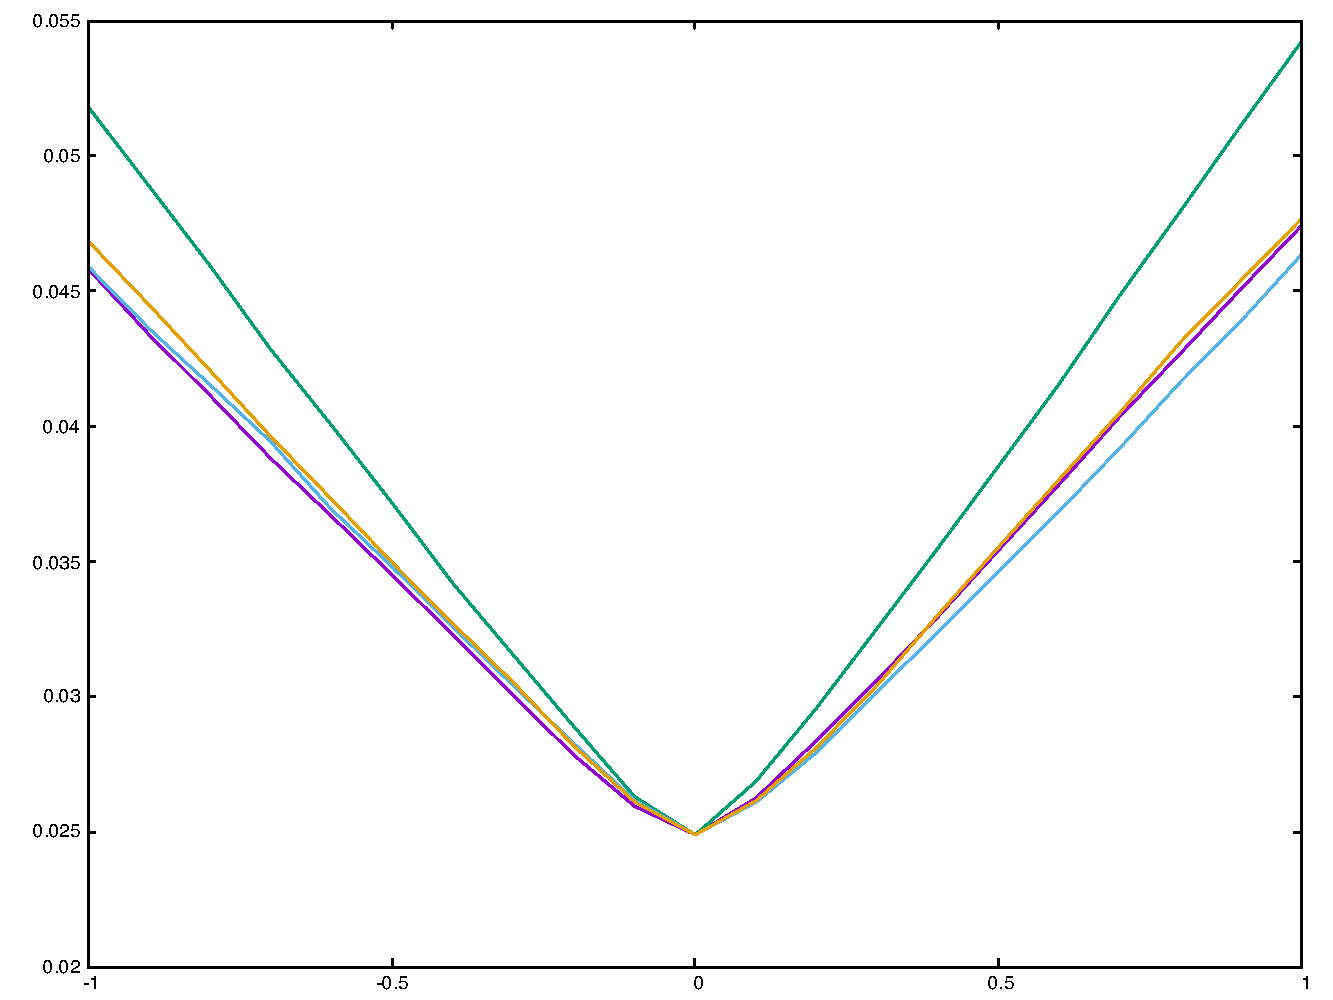
\includegraphics[width=\linewidth]{fig/ajherr/t3r/L_mae.pdf}
	\caption{L}
\end{subfigure}%
\begin{subfigure}{.33\textwidth}
	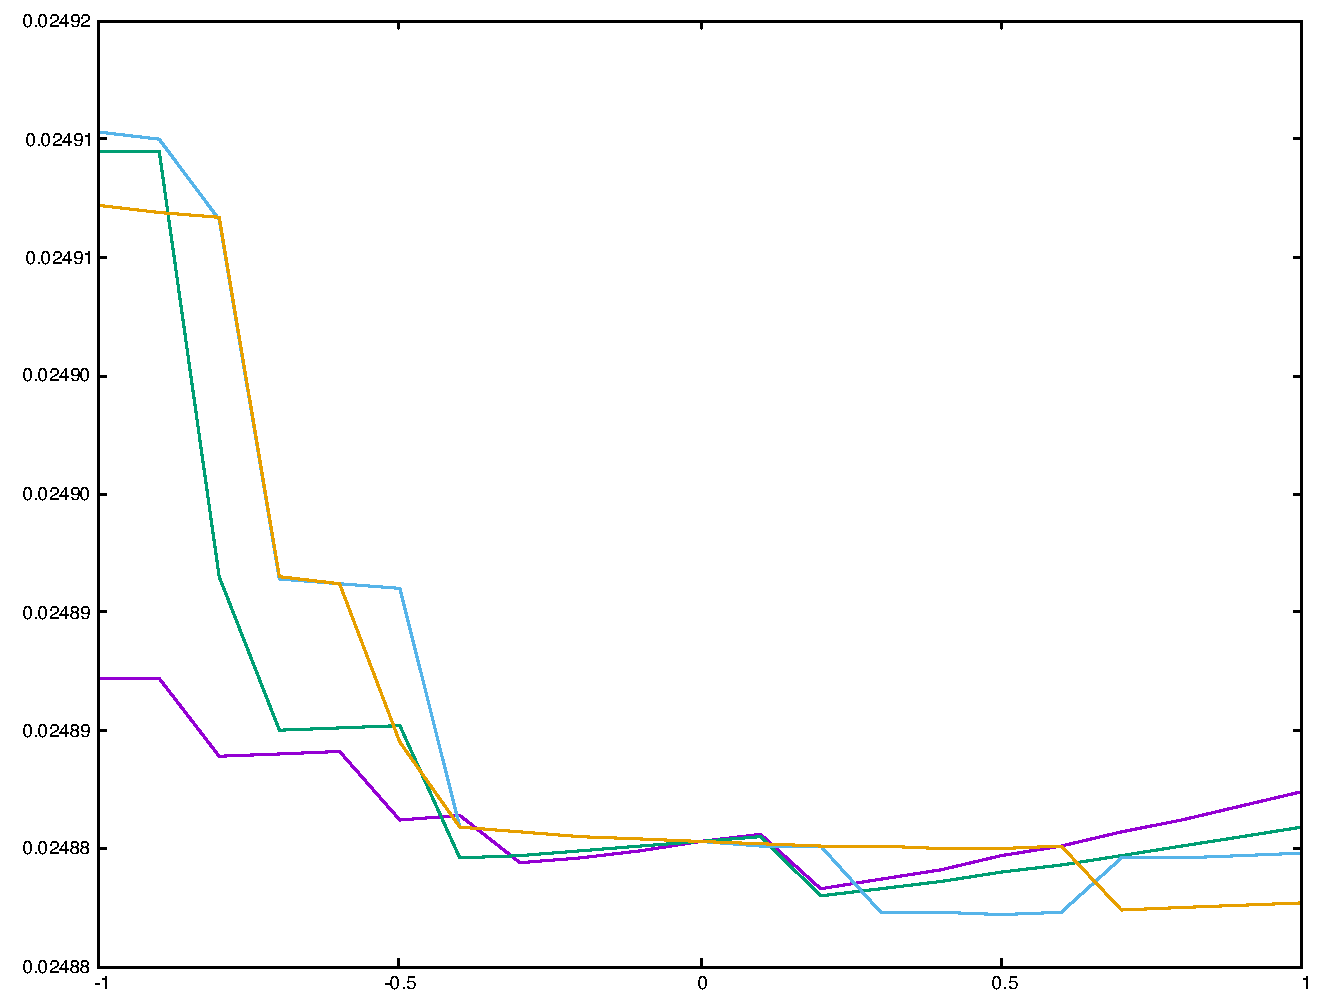
\includegraphics[width=\linewidth]{fig/ajherr/t3r/M_mae.pdf}
	\caption{M}
\end{subfigure}&
\begin{subfigure}{.33\textwidth}
	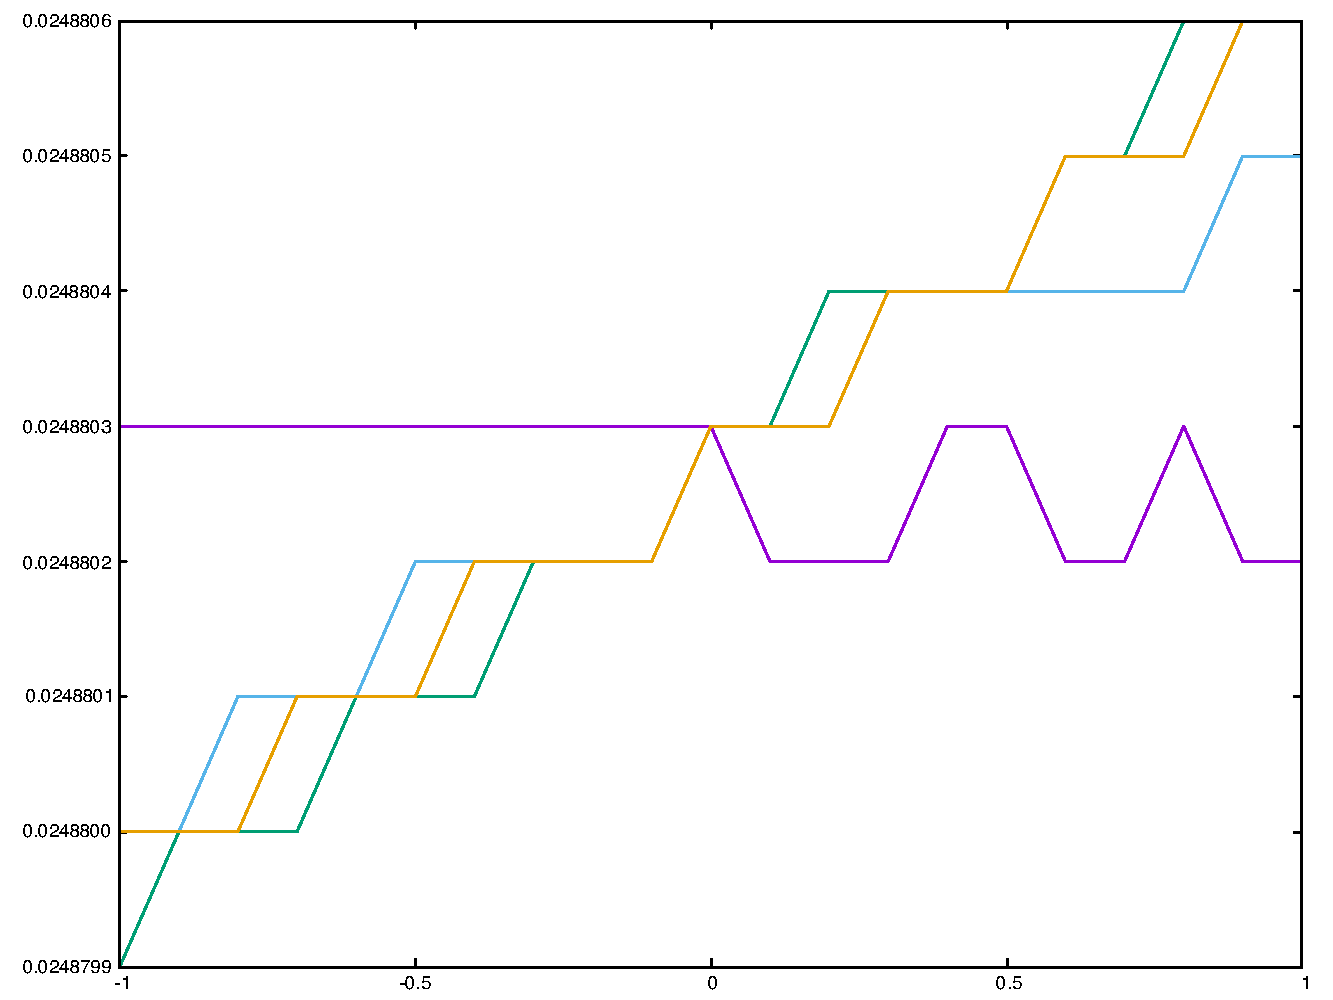
\includegraphics[width=\linewidth]{fig/ajherr/t3r/S_mae.pdf}
	\caption{S}
\end{subfigure}\\
\end{figure}


\paragraph{Observations} Again, no improvement of $e_{\chi}$ compared to mean absolute error.


\newpage

\subsection{Different resolutions, rejection}
Here, the same experiments are before are repeated, but the \gls{arcdh} is recorded, producing the $e_{r,\chi}$ error metric.


\subsubsection{Translation only}
Here only the translational part of the transformation is applied.

\begin{figure}[H]
\begin{subfigure}{.33\textwidth}
	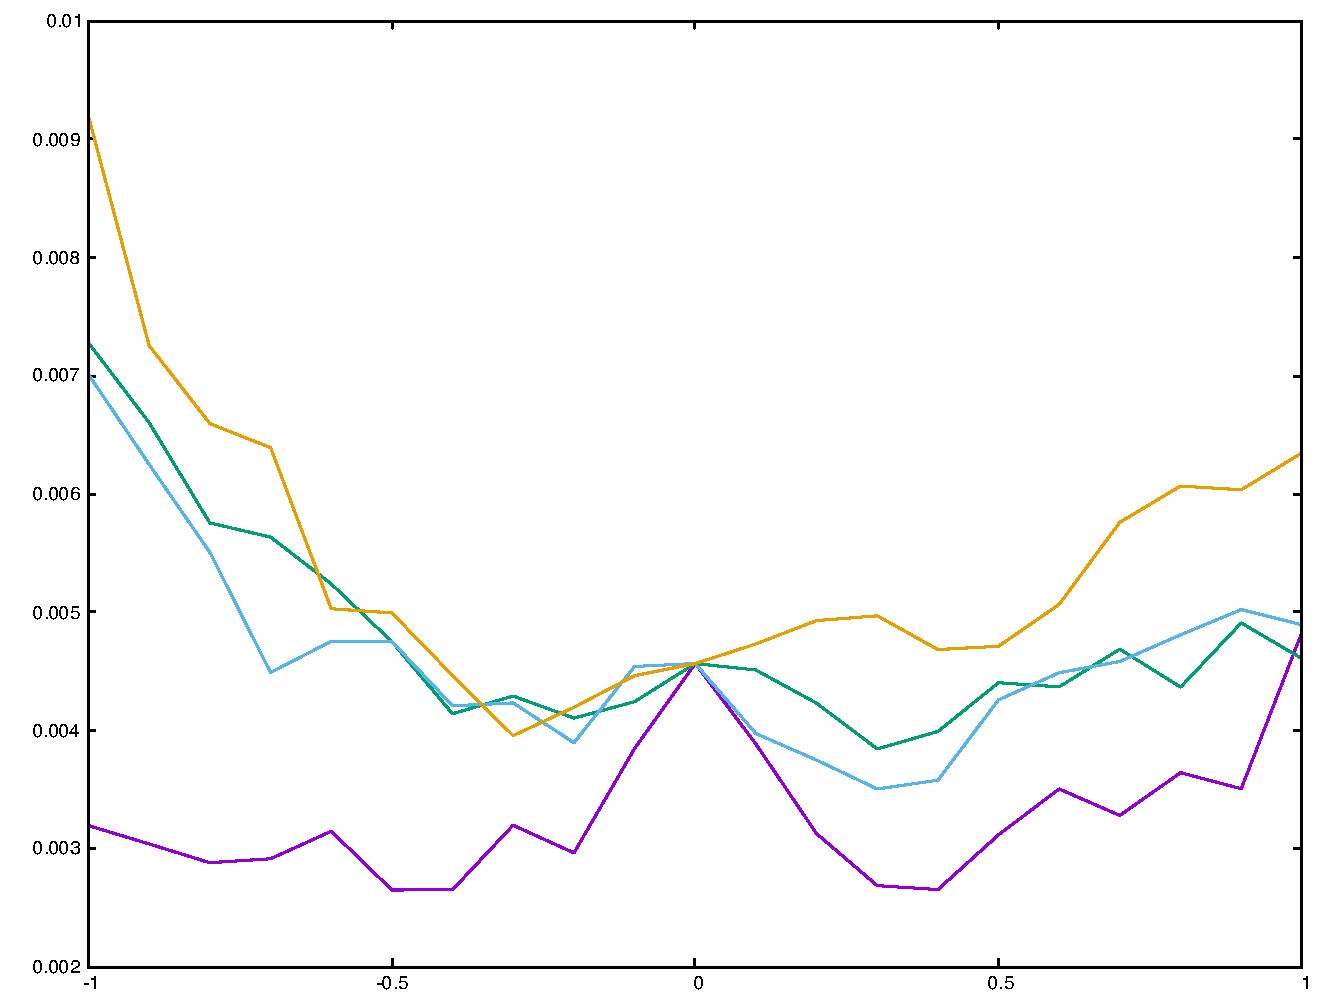
\includegraphics[width=\linewidth]{fig/ajherr/t3tr/L_chi.pdf}
\end{subfigure}%
\begin{subfigure}{.33\textwidth}
	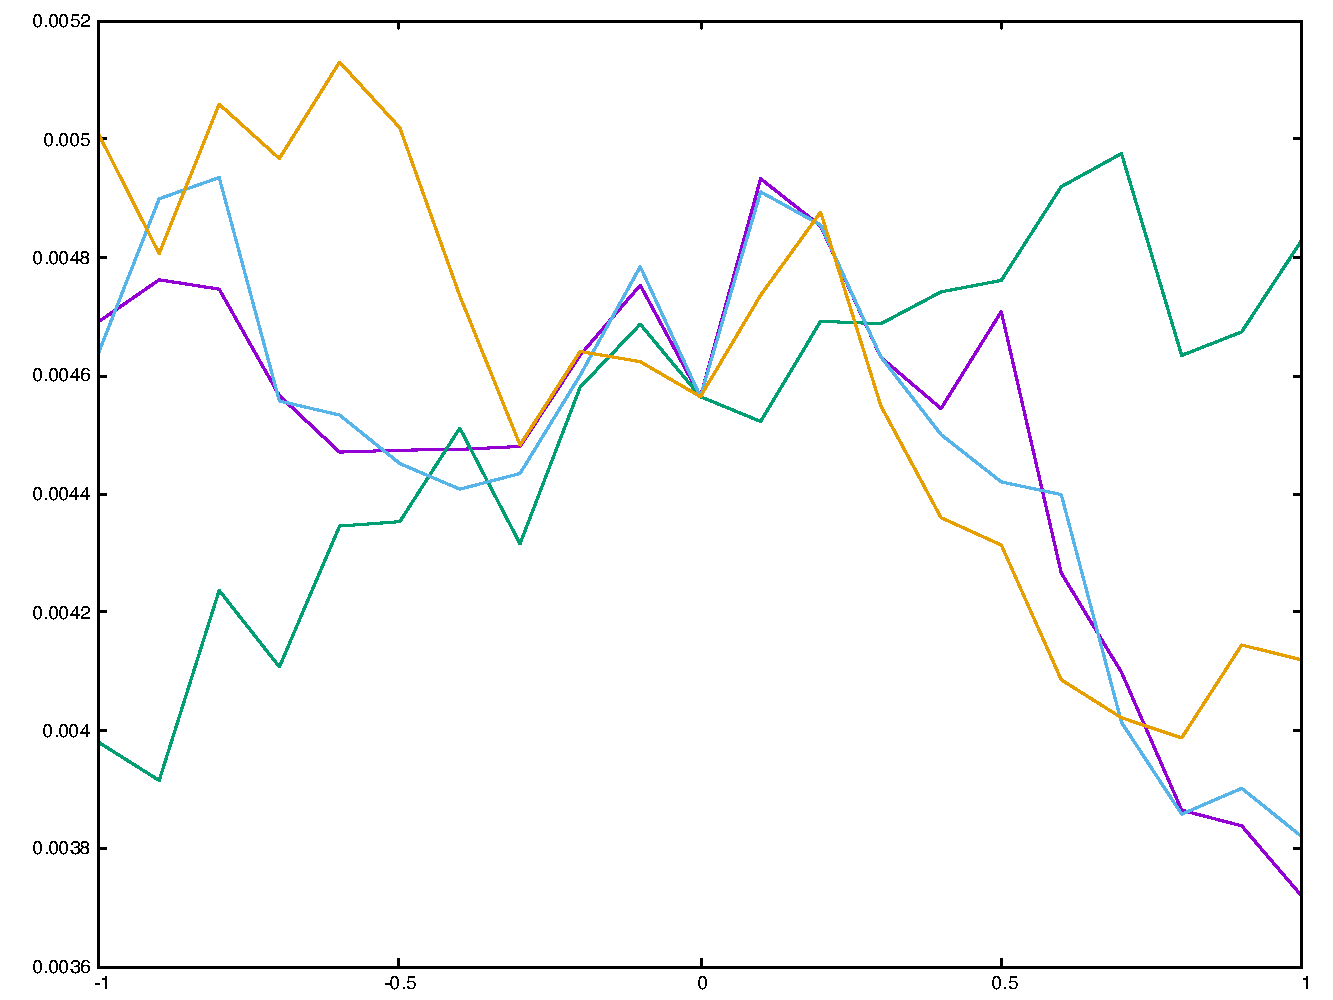
\includegraphics[width=\linewidth]{fig/ajherr/t3tr/M_chi.pdf}
\end{subfigure}&
\begin{subfigure}{.33\textwidth}
	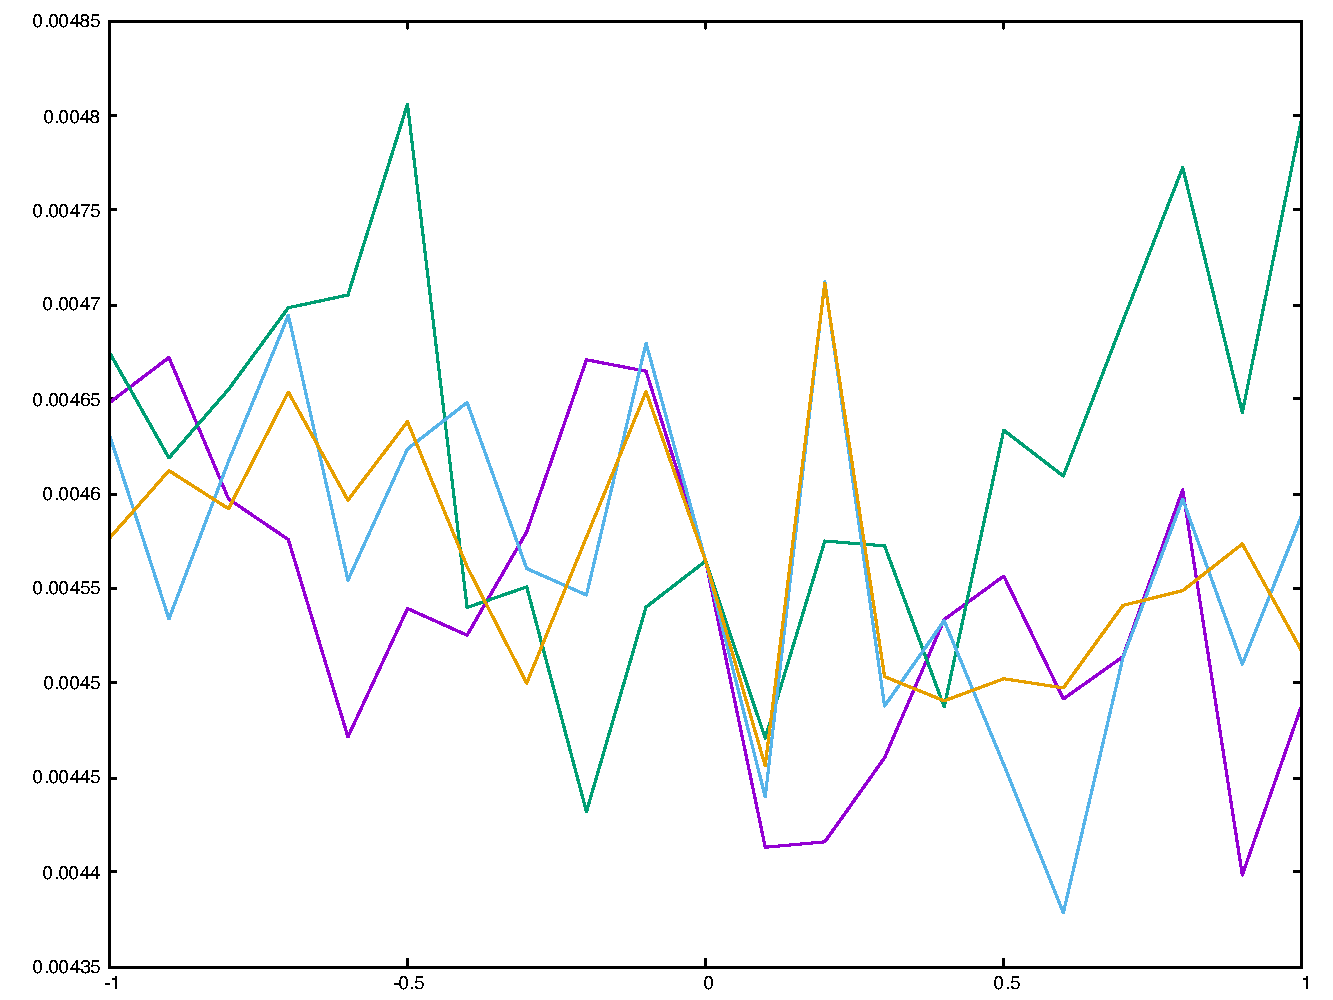
\includegraphics[width=\linewidth]{fig/ajherr/t3tr/S_chi.pdf}
\end{subfigure}\\
\begin{subfigure}{.33\textwidth}
	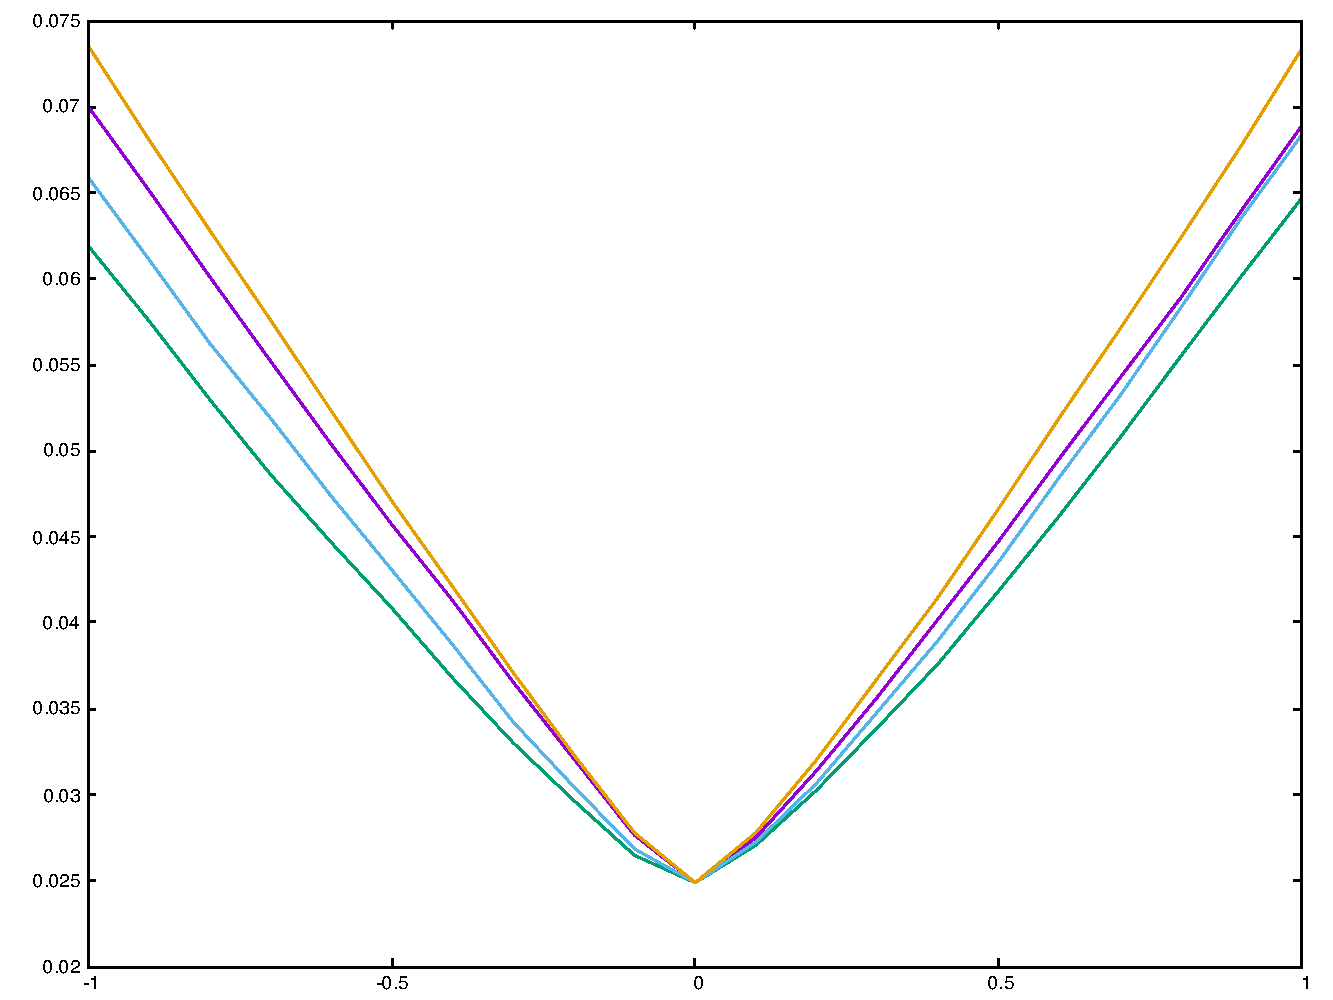
\includegraphics[width=\linewidth]{fig/ajherr/t3tr/L_mae.pdf}
	\caption{L}
\end{subfigure}%
\begin{subfigure}{.33\textwidth}
	\includegraphics[width=\linewidth]{fig/ajherr/t3tr/M_mae.pdf}
	\caption{M}
\end{subfigure}&
\begin{subfigure}{.33\textwidth}
	\includegraphics[width=\linewidth]{fig/ajherr/t3tr/S_mae.pdf}
	\caption{S}
\end{subfigure}\\
\end{figure}

\paragraph{Observations} Still, no improvement of $e_{r,\chi}$ compared to mean absolute error.



\subsubsection{Rotation only}
Now only the rotational part is applied.


\begin{figure}[H]
\begin{subfigure}{.33\textwidth}
	\includegraphics[width=\linewidth]{fig/ajherr/t3rr/L_chi.pdf}
\end{subfigure}%
\begin{subfigure}{.33\textwidth}
	\includegraphics[width=\linewidth]{fig/ajherr/t3rr/M_chi.pdf}
\end{subfigure}&
\begin{subfigure}{.33\textwidth}
	\includegraphics[width=\linewidth]{fig/ajherr/t3rr/S_chi.pdf}
\end{subfigure}\\
\begin{subfigure}{.33\textwidth}
	\includegraphics[width=\linewidth]{fig/ajherr/t3rr/L_mae.pdf}
	\caption{L}
\end{subfigure}%
\begin{subfigure}{.33\textwidth}
	\includegraphics[width=\linewidth]{fig/ajherr/t3rr/M_mae.pdf}
	\caption{M}
\end{subfigure}&
\begin{subfigure}{.33\textwidth}
	\includegraphics[width=\linewidth]{fig/ajherr/t3rr/S_mae.pdf}
	\caption{S}
\end{subfigure}\\
\end{figure}


\paragraph{Observations} At the L and M scales, no results can be observed. The two metrics at the S scale were recorded with more detail, because some result can be seen here: $e_{r,\chi}$ appears to converge towards a local minimum near the true transformation $\matr{M}$.

Because the curves represent values of the error metrics in cross sections of the rigid transformation space, they necessarily intersect at $x = 0$ which represents the true transformation. What is interesting about $e_{r,\chi}$ is that the curves have an inflection point at $x = 0$. The mean absolute error does not show this property.


\subsubsection{Rotation only, different centers}
To verify this, the following two plots were recorded the same way. The first one is recorded the same way as this last plot of $e_{r,\chi}$ at scale S, and again shows the local minimum at the true transformation $\matr{M}$.

On the second plot, the cross sections in the rigid transformation space were instead chosen to intersect at another random transformation located near the true transformation $\matr{M}$. Here the curves still intersect, but no local minimum can be observed.

This result may have been by chance. However, it shows that the inflection points of the curves are not a side effect of the interpolation in the transformations space at $t = 0$. It is were so, it would also be visible on the second plot.

\begin{figure}[H]
\begin{subfigure}{.49\textwidth}
	\includegraphics[width=\linewidth]{fig/ajherr/t3rr/c1.pdf}
	\caption{Centered on true transformation}
\end{subfigure}%
\begin{subfigure}{.49\textwidth}
	\includegraphics[width=\linewidth]{fig/ajherr/t3rr/c2.pdf}
	\caption{Centered on random transformation}
\end{subfigure}
\end{figure}





